\documentclass[11pt]{article}\usepackage[]{graphicx}\usepackage[]{color}
%% maxwidth is the original width if it is less than linewidth
%% otherwise use linewidth (to make sure the graphics do not exceed the margin)
\makeatletter
\def\maxwidth{ %
  \ifdim\Gin@nat@width>\linewidth
    \linewidth
  \else
    \Gin@nat@width
  \fi
}
\makeatother

\definecolor{fgcolor}{rgb}{0.345, 0.345, 0.345}
\newcommand{\hlnum}[1]{\textcolor[rgb]{0.686,0.059,0.569}{#1}}%
\newcommand{\hlstr}[1]{\textcolor[rgb]{0.192,0.494,0.8}{#1}}%
\newcommand{\hlcom}[1]{\textcolor[rgb]{0.678,0.584,0.686}{\textit{#1}}}%
\newcommand{\hlopt}[1]{\textcolor[rgb]{0,0,0}{#1}}%
\newcommand{\hlstd}[1]{\textcolor[rgb]{0.345,0.345,0.345}{#1}}%
\newcommand{\hlkwa}[1]{\textcolor[rgb]{0.161,0.373,0.58}{\textbf{#1}}}%
\newcommand{\hlkwb}[1]{\textcolor[rgb]{0.69,0.353,0.396}{#1}}%
\newcommand{\hlkwc}[1]{\textcolor[rgb]{0.333,0.667,0.333}{#1}}%
\newcommand{\hlkwd}[1]{\textcolor[rgb]{0.737,0.353,0.396}{\textbf{#1}}}%

\usepackage{framed}
\makeatletter
\newenvironment{kframe}{%
 \def\at@end@of@kframe{}%
 \ifinner\ifhmode%
  \def\at@end@of@kframe{\end{minipage}}%
  \begin{minipage}{\columnwidth}%
 \fi\fi%
 \def\FrameCommand##1{\hskip\@totalleftmargin \hskip-\fboxsep
 \colorbox{shadecolor}{##1}\hskip-\fboxsep
     % There is no \\@totalrightmargin, so:
     \hskip-\linewidth \hskip-\@totalleftmargin \hskip\columnwidth}%
 \MakeFramed {\advance\hsize-\width
   \@totalleftmargin\z@ \linewidth\hsize
   \@setminipage}}%
 {\par\unskip\endMakeFramed%
 \at@end@of@kframe}
\makeatother

\definecolor{shadecolor}{rgb}{.97, .97, .97}
\definecolor{messagecolor}{rgb}{0, 0, 0}
\definecolor{warningcolor}{rgb}{1, 0, 1}
\definecolor{errorcolor}{rgb}{1, 0, 0}
\newenvironment{knitrout}{}{} % an empty environment to be redefined in TeX

\usepackage{alltt}

\usepackage{amssymb}
\usepackage{amsmath}
\usepackage{bm}
\usepackage{graphicx}
\usepackage{hyperref}
\usepackage{url}
\usepackage{natbib}
\usepackage{epigraph}
\usepackage[utf8]{inputenc} % for UTF-8/single quotes from sQuote()

\usepackage{fancyvrb} % with VerbatimFootnotes, allow verb in footnotes
%\usepackage{listings}
\usepackage{array} % for ragged right table columns
% order of the next two matters
\usepackage[perpage,symbol]{footmisc}
\VerbatimFootnotes

\newcommand{\windows}{\textcircled{w}}
\newcommand{\code}[1]{{\tt #1}}
\newcommand{\flspecific}[1]{\emph{#1}}
%\bibliographystyle{ESA1009}

%\DeclareGraphicsExtensions{.jpg,.pdf,.mps,.png,.bmp}

% \setlength{\textwidth}{6.25in}
% \setlength{\textheight}{8.75in}
% \setlength{\evensidemargin}{0in}
% \setlength{\oddsidemargin}{0in}
% \setlength{\topmargin}{-.35in}
% \setlength{\parskip}{.1in}  
% \setlength{\parindent}{0.0in}  

% \numberwithin{equation}{chapter}
\pagestyle{headings}

\newcommand\R{{\sf R}}
\newcommand\Slang{{\sf S}}
\newcommand{\curRwver}{2013}

\newcommand{\curRver}{3.0.1}

\newcounter{exercise}
\numberwithin{exercise}{section}
\newcommand{\exnumber}{\addtocounter{exercise}{1} \theexercise \thinspace}

\newcommand{\prob}{\text{Prob}}


\sloppy
\title{An introduction to \R\ for modeling (lab 1)}
\date{\today}
\author{Stephen Ellner\thanks{Ecology and Evolutionary Biology,
    Cornell University}, modified by Ben Bolker and Steve Walker
  \thanks{Department of Mathematics \& Statistics and Biology,
    McMaster University}}

%% TODO: hint about range change in log graph
%% mfcol(,)
%% ?
\IfFileExists{upquote.sty}{\usepackage{upquote}}{}
\begin{document}

\maketitle

\includegraphics[width=2.64cm,height=0.93cm]{../icons/cc-attrib-nc.png}

\begin{minipage}[b]{3in}
{\small Licensed under the Creative Commons 
  attribution-noncommercial license
(\url{http://creativecommons.org/licenses/by-nc/3.0/}).
Please share \& remix noncommercially,
mentioning its origin.}
\end{minipage}

Version: 2014-09-03 17:33:23
  
\addtocounter{section}{-1}
\section{How to use this document}





\begin{itemize}
\item These notes contain many sample calculations. It is important to 
do these yourself---\textbf{type them in at your keyboard and see what
happens on your screen}---to get the 
feel of working in \R. 
\item \textbf{Exercises} in the middle of a section should be done
immediately when you get to them, and make sure you have them right 
before moving on. Some more challenging exercises 
(indicated by asterisks) appear at the end of some sections. These
can be left until later, and will be assigned as homework.   
\end{itemize}

These notes are based in part on course materials by former TAs
Colleen Webb, Jonathan Rowell and Daniel Fink at Cornell, Professors
Lou Gross (University of Tennessee) and Paul Fackler (NC State
University), and on the book \emph{Getting Started with Matlab} by
Rudra Pratap (Oxford University Press).  They also draw on the
documentation supplied with \R.  They parallel, but go into 
more depth than, the chapter supplement for the book
\emph{Ecological Models and Data in \R} by Ben Bolker (Princeton University Press).

You can find many other similar introductions scattered around the
web, or in the ``contributed documentation'' section on the R web site
(\url{http://cran.r-project.org/other-docs.html}).  This particular
version is limited (it has similar coverage to Sections~1 and 2 of the
\emph{Introduction to \R} that comes with \R).

\section{What is \R?}
\R\ is an object-oriented scripting language that combines 
\begin{itemize}
\item a programming language called \Slang,
developed by John Chambers at Bell Labs, that can be used for 
numerical simulation of deterministic and stochastic dynamic models
\item an extensive set of functions for classical and modern
  statistical data analysis and modeling
\item graphics functions for visualizing data and model output
\item a user interface with a few basic menus and extensive help
facilities
\end{itemize}

\R\ is an open source project, available for free download via the
Web. Originally a research project in statistical computing
\citep{IhakaGentleman1996}, it is now managed by a development team
that includes a number of well-regarded statisticians, and is widely
used by statistical researchers (and a growing number of theoretical
ecologists and ecological modelers) as a platform for making new
methods available to users. A standard installation of \R\ also
includes extensive documentation, including an introductory manual
($\approx 100$ pages) and a comprehensive reference manual (over 1000
pages).

\subsection{Installing \R\ and RStudio on your computer: basics}

If \R\ and RStudio are already installed on your computer, 
you can skip this section.

Here are the instructions:
\begin{itemize}
\item go to \url{http://www.rstudio.com/ide/download/desktop}
\item if you don't yet have \R, follow the link at the end of this
  sentence: \emph{RStudio requires R 2.11.1 (or higher). If you don't already have R, you can download it here.}
\begin{itemize}
  \item click on the download corresponding to your operating system
  \item click on R-3.1.1-snowleopard.pkg or R-3.1.1-mavericks.pkg if
    you are on a Mac and the link that says \emph{install R for the
      first time} if you are on Windows.
\item read and follow
the instructions (which are pretty much ``click on the icon'').
\end{itemize}
\item go back to \url{http://www.rstudio.com/ide/download/desktop}
 \item click on the download most appropriate for your system
 \item read and follow instructions
\end{itemize}

\R\ should work well on any reasonably modern computer.
R moves quickly: if possible, you should make
sure you have upgraded to the most recent version
available, or at least that your version isn't more
than about a year old.

% \flspecific{
% You can also use one of the CDs I've burned for the class. 
% These CDs also contain
% pre-compiled versions of a large number of packages
% from CRAN, as well as a variety of other tools and documents.}

The standard distributions of \R\ include several \emph{packages},
user-contributed suites of add-on functions (unfortunately, the
command to load a package into \R\ is \code{library}!).  These
Notes use some packages that are not part of the standard
distribution. In general, you can install additional packages 
from within \R\ using the \code{Packages} menu,
or the \code{install.packages} command.
(See below.)

%\windows\ It may also be a good idea to move \R's default
%directory \ldots


\section{Interactive calculations}

When you start RStudio it opens the \textbf{console} window.
The console has a few basic menus at the top; check them out on your own. The console is 
also where you enter commands for \R\ to execute
\emph{interactively}, meaning that the command is executed and 
the result is displayed as soon as you hit the \code{ Enter} key. For example, at 
the command prompt \code{>}, type in \code{2+2} and hit \code{Enter}; you will see 
\begin{knitrout}
\definecolor{shadecolor}{rgb}{0.969, 0.969, 0.969}\color{fgcolor}\begin{kframe}
\begin{alltt}
\hlstd{> }\hlnum{2} \hlopt{+} \hlnum{2}
\end{alltt}
\begin{verbatim}
## [1] 4
\end{verbatim}
\end{kframe}
\end{knitrout}
\noindent (When cutting and pasting from this document to \R, don't include the
text for the command prompt (\code{>}).)

To do anything complicated, you have to store the results from
calculations by \emph{assigning} them to variables, using \code{=} or
\verb+<-+. For example:
\begin{knitrout}
\definecolor{shadecolor}{rgb}{0.969, 0.969, 0.969}\color{fgcolor}\begin{kframe}
\begin{alltt}
\hlstd{> }\hlstd{a} \hlkwb{<-} \hlnum{2} \hlopt{+} \hlnum{2}
\end{alltt}
\end{kframe}
\end{knitrout}
\noindent \R\ automatically creates the variable \code{a} and stores the result (4)
in it, but it doesn't print anything.  This may seem strange, but you'll
often be creating and manipulating huge sets of data that would fill
many screens, so the default is to skip printing the results.
To ask \R\ to print the value, just type the variable name by itself
at the command prompt:
\begin{knitrout}
\definecolor{shadecolor}{rgb}{0.969, 0.969, 0.969}\color{fgcolor}\begin{kframe}
\begin{alltt}
\hlstd{> }\hlstd{a}
\end{alltt}
\begin{verbatim}
## [1] 4
\end{verbatim}
\end{kframe}
\end{knitrout}
\noindent (the \code{[1]} at the beginning of the line is just \R\ printing
an index of element numbers; if you print a result that
displays on multiple lines, \R\ will put an index at the beginning
of each line.  \code{print(a)} also works to print the value of
a variable.)  By default, a variable created this way is a \emph{vector}, 
and it is \emph{numeric} because we gave \R\ a number rather
than some other type of data (e.g. a character string like \code{"pxqr"}).
In this case \code{a} is a numeric vector of length 1,
which acts just like a number. 

You could also type \code{a <- 2 + 2; a},
using a semicolon to put two or more commands on a single line.
Conversely, you can break lines \emph{anywhere that \R\ can tell you haven't
finished your command} and \R\ will give you a ``continuation'' prompt
(\code{+}) to let you know that it doesn't think you're finished yet: try typing
\begin{knitrout}
\definecolor{shadecolor}{rgb}{0.969, 0.969, 0.969}\color{fgcolor}\begin{kframe}
\begin{alltt}
\hlstd{> }\hlstd{a} \hlkwb{=} \hlnum{3} \hlopt{*} \hlstd{(}\hlnum{4} \hlopt{+}
\hlstd{+  }\hlnum{5}\hlstd{)}
\end{alltt}
\end{kframe}
\end{knitrout}
\noindent to see what happens (you will sometimes see the continuation prompt
when you don't expect it, e.g. if you forget to close parentheses).
If you get stuck continuing a command you don't want---e.g. you opened
the wrong parentheses---just hit the \code{Escape} key or the stop
icon in the menu bar to get out.

Variable names in \R\ must begin with a letter, followed by letters or numbers.
You can break up long names with a period, as in
\code{very.long.variable.number.3}, or an underscore (\code{\_}), but you 
can't use blank spaces in variable names
(or at least it's not worth the trouble).
Variable names in \R\ are case sensitive,
so \code{Abc} and \code{abc} 
are different variables.
Make variable names long enough to remember, short
enough to type.
\code{N.per.ha} or \code{pop.density} are better than \code{x}
and \code{y} (too short) or \code{available.nitrogen.per.hectare} (too long).
Avoid \code{c}, \code{l}, \code{q}, \code{t}, \code{C}, \code{D},
\code{F}, \code{I}, \code{O}, and \code{T}, which are either built-in \R\ functions or
hard to tell apart from other symbols (e.g. \code{l} (lower-case L) vs. \code{1} (numeral 1)).

\R\ does calculations with variables as if they were numbers. It uses  
\code{+}, \code{-}, \code{*}, \code{/}, and \verb!^!
for addition, subtraction, multiplication, division and 
exponentiation, respectively. For example:
% emphasis on semicolons seemed unnecessary
\begin{knitrout}
\definecolor{shadecolor}{rgb}{0.969, 0.969, 0.969}\color{fgcolor}\begin{kframe}
\begin{alltt}
\hlstd{> }\hlstd{x} \hlkwb{<-} \hlnum{5}
\hlstd{> }\hlstd{y} \hlkwb{<-} \hlnum{2}
\hlstd{> }\hlstd{z1} \hlkwb{<-} \hlstd{x}\hlopt{*}\hlstd{y}  \hlcom{## no output}
\hlstd{> }\hlstd{z2} \hlkwb{<-} \hlstd{x}\hlopt{/}\hlstd{y}  \hlcom{## no output}
\hlstd{> }\hlstd{z3} \hlkwb{<-} \hlstd{x}\hlopt{^}\hlstd{y}  \hlcom{## no output}
\hlstd{> }\hlstd{z2}
\end{alltt}
\begin{verbatim}
## [1] 2.5
\end{verbatim}
\begin{alltt}
\hlstd{> }\hlstd{z3}
\end{alltt}
\begin{verbatim}
## [1] 25
\end{verbatim}
\end{kframe}
\end{knitrout}
\noindent Even though \R\ did not display the values of \code{x} and \code{y}, it ``remembers'' that 
it assigned values to them. Type \code{x; y} to display the values. 

You can retrieve and edit previous commands.
The up-arrow (\thinspace $\uparrow$ \thinspace) key (or
\code{Control-P}) recalls previous 
commands to the prompt. For example, you can bring back the second-to-last command and edit it to
\begin{knitrout}
\definecolor{shadecolor}{rgb}{0.969, 0.969, 0.969}\color{fgcolor}\begin{kframe}
\begin{alltt}
\hlstd{> }\hlstd{z3} \hlkwb{<-} \hlnum{2}\hlopt{*}\hlstd{x}\hlopt{^}\hlstd{y}
\end{alltt}
\end{kframe}
\end{knitrout}
\noindent (experiment with the other arrow keys ($\downarrow$, $\rightarrow$, $\leftarrow$), \code{Home} and \code{End} keys
too).
This will save you many hours in the long run.

You can combine several operations in one calculation:
\begin{knitrout}
\definecolor{shadecolor}{rgb}{0.969, 0.969, 0.969}\color{fgcolor}\begin{kframe}
\begin{alltt}
\hlstd{> }\hlstd{A} \hlkwb{<-} \hlnum{3}
\hlstd{> }\hlstd{C} \hlkwb{<-} \hlstd{(A} \hlopt{+} \hlnum{2} \hlopt{*} \hlkwd{sqrt}\hlstd{(A))} \hlopt{/} \hlstd{(A} \hlopt{+} \hlnum{5} \hlopt{*} \hlkwd{sqrt}\hlstd{(A)); C}
\end{alltt}
\begin{verbatim}
## [1] 0.5544
\end{verbatim}
\end{kframe}
\end{knitrout}
\noindent Parentheses specify the order of operations. 
The command
\begin{knitrout}
\definecolor{shadecolor}{rgb}{0.969, 0.969, 0.969}\color{fgcolor}\begin{kframe}
\begin{alltt}
\hlstd{> }\hlstd{C} \hlkwb{<-} \hlstd{A} \hlopt{+} \hlnum{2} \hlopt{*} \hlkwd{sqrt}\hlstd{(A)} \hlopt{/} \hlstd{A} \hlopt{+} \hlnum{5} \hlopt{*} \hlkwd{sqrt}\hlstd{(A)}
\end{alltt}
\end{kframe}
\end{knitrout}
\noindent is not the same as the one above; rather, it is 
equivalent to \code{C <- A + 2*(sqrt(A)/A) + 5*sqrt(A)}.

The default order of operations is: (1) parentheses; 
(2) exponentiation, or powers, (3) multiplication 
and division, (4) addition and subtraction (``\textbf{p}retty \textbf{p}lease
\textbf{e}xcuse \textbf{m}y \textbf{d}ear \textbf{A}unt \textbf{S}ally'').

\begin{tabular}{lcl}
\verb!b  <-  12-4/2^3! & gives  & \verb!12 - 4/8 = 12 - 0.5 = 11.5! \\
\verb!b  <-  (12-4)/2^3! & gives & \verb!8/8 = 1! \\
\verb!b  <-  -1^2!   &          gives  &  \verb!-(1^2) = -1! \\
\verb!b  <-  (-1)^2! &          gives  &  \verb!1!
\end{tabular} 

In complicated expressions 
you might start off by \emph{using parentheses to specify 
explicitly what you want}, such as \verb! b  <-  12 - (4/(2^3)) ! 
or at least \verb! b  <-  12 - 4/(2^3) !; a few extra sets of parentheses
never hurt anything, although when you get confused
it's better to think through the order of operations rather than flailing
around adding parentheses at random.

\R\ also has many \emph{built-in mathematical functions} that operate on variables
(Table \ref{MathFunctions} shows a few). 


\begin{table}[t]
\begin{tabular}{p{140pt}p{290pt}}
\hline
\code{abs} & absolute value \\
\code{cos}, \code{sin}, \code{tan} &  cosine, sine, tangent of angle $x$ in radians\\
\code{exp}  & exponential function, $e^x$  \\
\code{log}  & natural (base-$e$) logarithm \\
\code{log10} &  common (base-10) logarithm \\
\code{sqrt}  &  square root \\
\hline 
\end{tabular}
\caption{Some of the built-in mathematical functions in \R. You can
get a more complete list from the Help system: \code{?Arithmetic} for simple, 
\code{?log} for logarithmic, \code{?sin} for trigonometric, and \code{?Special} for special 
functions.} 
\label{MathFunctions}
\end{table}

\textbf{Exercise\exnumber}: Using editing
shortcuts wherever you can, have \R\ compute the values of 
\begin{enumerate}
\item $\frac{2^7}{2^7 - 1}$
and compare it with 
$( {1 - \frac{1}{2^7}} )^{-1}$
(If any square brackets [] show up in your web browser's
rendition of these equations, replace
them with regular parentheses ().)
\item 
\begin{itemize}
\item $1+0.2$
\item $1+0.2+0.2^2/2$
\item $1+0.2+0.2^2/2+0.2^3/6$
\item $e^{0.2}$ (remember that \R\ knows \code{exp} but not $e$;
how would you get \R\ to tell you the value of $e$?  What is the
point of this exercise?)
\end{itemize}
\item{the standard normal probability density,
$\frac{1}{\sqrt{2 \pi}} e^{-x^2/2}$, for values of $x=1$
and $x=2$ (\R\ knows $\pi$ as \code{pi}.)
(You can check your answers against the built-in function
for the normal distribution; \code{dnorm(1)} and
\code{dnorm(2)} should give
you the values for the standard normal for $x=1$ and $x=2$.)}
\end{enumerate}

\section{The help system}

\R\ has a help system, although it is generally
better for providing detail or reminding you how to do things than
for basic ``how do I \ldots?'' questions.

\begin{itemize}
\item You can get help on any \R\ function by entering
\begin{verbatim}
?foo
\end{verbatim} 
(where \code{foo} is the name of the function
you are interested in)
in the console window (e.g., try \code{?sin}). 
\item The \code{Help} menu on the tool bar
provides links to other documentation,
including the manuals and FAQs, and a 
Search facility (`Apropos' on the menu)
which is useful if you sort of maybe remember part of the
the name of what it is you need help on.
\item Typing \code{help.start()}
opens a web browser with help information.
\item \code{example(cmd)} will run any examples that are included
in the help page for command \code{cmd}.
\item{\code{demo(topic)} runs demonstration code on topic \code{topic}: type
\code{demo()} by itself to list all available demos}
\end{itemize}

By default, \R's help system only provides information 
about functions that are in the base system and packages
that you have loaded with \code{library} (see below).
\begin{itemize}
\item \code{??topic} or \code{help.search("topic")} 
  (with quotes)
will list information
related to \code{topic} available in the base system 
or in any extra installed packages:
then use \code{?topic} to see the information, perhaps using
\code{library(pkg)} to load the appropriate package first.
\code{help.search} uses ``fuzzy matching'' --- for example, 
\code{help.search("log")} finds 528 entries (on my
particular system) including lots of
functions with ``plot'', which includes the letters ``lot'', which
are \emph{almost} like ``log''.  If you can't stand it, you
can turn this behavior off by specifying the incantation
\code{help.search("log",agrep=FALSE)} (81 results which still include
matches for ``logistic'', ``myelogenous'', and ``phylogeny'' \ldots)
\item \code{help(package="pkg")} will list all the help pages for
a loaded package.
\item \code{example(fun)} will run the examples (if any) given
  in the help for a particular function \code{fun}: e.g. \code{example(log)}
\item \code{RSiteSearch("topic")} does a full-text
  search of all the \R\ documentation and the mailing list archives
  for information on \code{topic} (you need an active
  internet connection).  
\item the \code{sos} package is a web-aware help function that
  searches all of the packages on CRAN; its \code{findFn} function
  tries to find and organize functions in any package on CRAN that
  match a search string (again, you need a network connection for this).
\end{itemize}

Try out one or
more of these aspects of the help system.

% Finally, here's a commentary on the
% help system in \R\ from Graham Lawrence:
% \begin{quote}
% \small
% I hate to say this, but what really helped me the most, after the initial
% feet-wetting, was to abandon the help manuals.  Searching manuals for the
% answer to a specific question is frustrating because one does not know the
% key term for the search engine to deliver the item needed.

% So I stopped being serious and production oriented and simply played with \R\ 
% for a couple of months.  Open the Base package, scan the list of contents
% for titles that pique my curiosity, paste their examples into \R\ and see what
% happens.  And those examples use other functions and their documentation has
% more examples and so on and on; and pretty soon after, whoops, there's
% another afternoon gone down the tubes.  But all this apparent time wasting
% had a most happy result.  I now find, much more often than not, that I know
% what I need to look up to answer a specific question, and that does wonders
% for my disposition.

% I think of \R\ as a vast jungle, criss-crossed with myriad game trails (the
% documentation to each function in the packages).  And I can explore each
% trail and see what animal it leads to in its native habitat, by pasting the
% examples into \R\ and examining the result.  So when I see an interesting
% spoor or paw print, I take a stroll down that trail and see where it leads.
% Not the most efficient way of learning the language, no doubt, but a
% pleasant and interesting entertainment rather than a chore.
% \end{quote}

\textbf{Exercise\exnumber}: Do an Apropos on \code{sin} via the Help
menu, to see what it does. Now enter the command
\begin{knitrout}
\definecolor{shadecolor}{rgb}{0.969, 0.969, 0.969}\color{fgcolor}\begin{kframe}
\begin{alltt}
\hlstd{> }\hlkwd{help.search}\hlstd{(}\hlstr{"sin"}\hlstd{)}
\end{alltt}
\end{kframe}
\end{knitrout}
\noindent and see what that does (answer: \code{help.search} pulls up
all help pages that include `sin' anywhere in their title or
text. Apropos just looks at the name of the function).

\section{A first interactive session: a ``leaky bucket'' model}

\newcommand{\rmax}{r_{\mbox{\small max}}}
To get a feel for working in \R\ we'll construct a simple discrete-time
dynamical system, sometimes known as the ``leaky bucket'' model.

Suppose that in a queue (a group of people or things waiting for service --- e.g. people
waiting at a bank, or jobs waiting for processing on a computer system, or cars
in line at a toll booth), 25\% (rounded) of
the people waiting are served every hour and 10 new people arrive every hour.
(For precision, we will assume that the 10 new people arrive at the \emph{end}
of the hour and are not counted in the fraction served.)

Suppose the queue is initially empty.  We could run this model by brute force by
typing
\begin{knitrout}
\definecolor{shadecolor}{rgb}{0.969, 0.969, 0.969}\color{fgcolor}\begin{kframe}
\begin{alltt}
\hlstd{> }\hlstd{N} \hlkwb{<-} \hlnum{0}
\end{alltt}
\end{kframe}
\end{knitrout}
\noindent to set the initial state and then typing (or cutting and
pasting)
\begin{knitrout}
\definecolor{shadecolor}{rgb}{0.969, 0.969, 0.969}\color{fgcolor}\begin{kframe}
\begin{alltt}
\hlstd{> }\hlstd{N} \hlkwb{<-} \hlstd{N} \hlopt{-} \hlkwd{round}\hlstd{(}\hlnum{0.25} \hlopt{*} \hlstd{N)}
\hlstd{> }\hlstd{N} \hlkwb{<-} \hlstd{N} \hlopt{+} \hlnum{10}
\end{alltt}
\end{kframe}
\end{knitrout}
\noindent over and over again.

Of course, this would be extremely tedious (we also wouldn't see the 
results unless we typed \code{N} by itself from time to time
to see where we'd gotten).  This approach doesn't save the results
over time; we can only see the current state of the system.

Suppose that we decide we want to run the system for 20 steps.
We can set aside space for a vector of 20 numbers, set the
first to zero, and assign a variable \code{i} as a counter
(if \code{i} is an integer in the correct range,
then \code{N[i]} refers to the \code{i}\textsuperscript{th}
value from the vector \code{N} --- more on this below):
\begin{knitrout}
\definecolor{shadecolor}{rgb}{0.969, 0.969, 0.969}\color{fgcolor}\begin{kframe}
\begin{alltt}
\hlstd{> }\hlstd{N} \hlkwb{<-} \hlkwd{numeric}\hlstd{(}\hlnum{20}\hlstd{)}
\hlstd{> }\hlstd{N[}\hlnum{1}\hlstd{]} \hlkwb{<-} \hlnum{0}
\hlstd{> }\hlstd{i} \hlkwb{<-} \hlnum{1}
\end{alltt}
\end{kframe}
\end{knitrout}
\noindent Then we can do the following steps repeatedly:
\begin{knitrout}
\definecolor{shadecolor}{rgb}{0.969, 0.969, 0.969}\color{fgcolor}\begin{kframe}
\begin{alltt}
\hlstd{> }\hlstd{i} \hlkwb{<-} \hlstd{i}\hlopt{+}\hlnum{1}
\hlstd{> }\hlstd{N[i]} \hlkwb{<-} \hlstd{N[i}\hlopt{-}\hlnum{1}\hlstd{]}\hlopt{-}\hlkwd{round}\hlstd{(}\hlnum{0.25}\hlopt{*}\hlstd{N[i}\hlopt{-}\hlnum{1}\hlstd{])}\hlopt{+}\hlnum{10}  \hlcom{## condense}
\end{alltt}
\end{kframe}
\end{knitrout}
\noindent Of course, this doesn't help much in the tedium department.
We should instead use a \code{while} statement:
\begin{knitrout}
\definecolor{shadecolor}{rgb}{0.969, 0.969, 0.969}\color{fgcolor}\begin{kframe}
\begin{alltt}
\hlstd{> }\hlstd{i} \hlkwb{<-} \hlnum{1}
\hlstd{> }\hlkwa{while} \hlstd{(i}\hlopt{<}\hlnum{20}\hlstd{) \{}
\hlstd{+  }  \hlstd{i} \hlkwb{<-} \hlstd{i}\hlopt{+}\hlnum{1}
\hlstd{+  }  \hlstd{N[i]} \hlkwb{<-} \hlstd{N[i}\hlopt{-}\hlnum{1}\hlstd{]}\hlopt{-}\hlkwd{round}\hlstd{(}\hlnum{0.25}\hlopt{*}\hlstd{N[i}\hlopt{-}\hlnum{1}\hlstd{])}\hlopt{+}\hlnum{10}
\hlstd{+  }\hlstd{\}}
\hlstd{> }\hlstd{N}
\end{alltt}
\begin{verbatim}
##  [1]  0 10 18 24 28 31 33 35 36 37 38 38 38 38 38 38 38 38
## [19] 38 38
\end{verbatim}
\end{kframe}
\end{knitrout}
\noindent R repeatedly tests the \emph{condition} \verb+i<20+ given
in parentheses after \code{while}; if it is true, it runs
all of the code inside the
curly brackets (\verb+{}+), then starts again.

\textbf{Exercise\exnumber}: Why did we use the 
condition \verb+i < 20+ rather than the condition
\verb+i <= 20+?

Alternatively, since we know in advance how many times
we want to run the model, we can instead use a ``\code{for}
loop'':
\begin{knitrout}
\definecolor{shadecolor}{rgb}{0.969, 0.969, 0.969}\color{fgcolor}\begin{kframe}
\begin{alltt}
\hlstd{> }\hlkwa{for} \hlstd{(i} \hlkwa{in} \hlnum{2}\hlopt{:}\hlnum{20}\hlstd{) \{}
\hlstd{+  }  \hlstd{N[i]} \hlkwb{<-} \hlstd{N[i} \hlopt{-} \hlnum{1}\hlstd{]} \hlopt{-} \hlkwd{round}\hlstd{(}\hlnum{0.25} \hlopt{*} \hlstd{N[i} \hlopt{-} \hlnum{1}\hlstd{])} \hlopt{+} \hlnum{10}
\hlstd{+  }\hlstd{\}}
\hlstd{> }\hlstd{N}
\end{alltt}
\begin{verbatim}
##  [1]  0 10 18 24 28 31 33 35 36 37 38 38 38 38 38 38 38 38
## [19] 38 38
\end{verbatim}
\end{kframe}
\end{knitrout}
\noindent The colon (:) operator creates a sequence of integers
starting at 2 and ending at 20 (notice that we start from 1, not 2,
because we have already set the value for \code{N[1]}).  For each
value in this vector, R sets the loop variable \code{i} to that value
and runs the code inside the curly brackets.

Let's plot the results.  \code{plot(N)} by itself will plot the values
in \code{N} on the $y$-axis against their ``index'' (position in the
vector) on the $x$-axis, but it might be better to specify the $x$
values explicitly, as in \code{plot(1:20,N)}.  Perhaps even better, we
can assign the $x$ values to a variable: at the same time, we can (1)
specify that R should use both lines and points to plot the values by
specifying \code{type="b"} and (2) specify more informative labels for
the axes (see Figure~\ref{fig:queue1}).
\begin{knitrout}
\definecolor{shadecolor}{rgb}{0.969, 0.969, 0.969}\color{fgcolor}\begin{kframe}
\begin{alltt}
\hlstd{> }\hlstd{tvec} \hlkwb{<-} \hlnum{1}\hlopt{:}\hlnum{20}
\hlstd{> }\hlkwd{plot}\hlstd{(tvec, N,} \hlkwc{type} \hlstd{=} \hlstr{"b"}\hlstd{,}
\hlstd{+  }     \hlkwc{xlab} \hlstd{=} \hlstr{"Time (hours)"}\hlstd{,}
\hlstd{+  }     \hlkwc{ylab} \hlstd{=} \hlstr{"Queue length"}\hlstd{)}
\end{alltt}
\end{kframe}
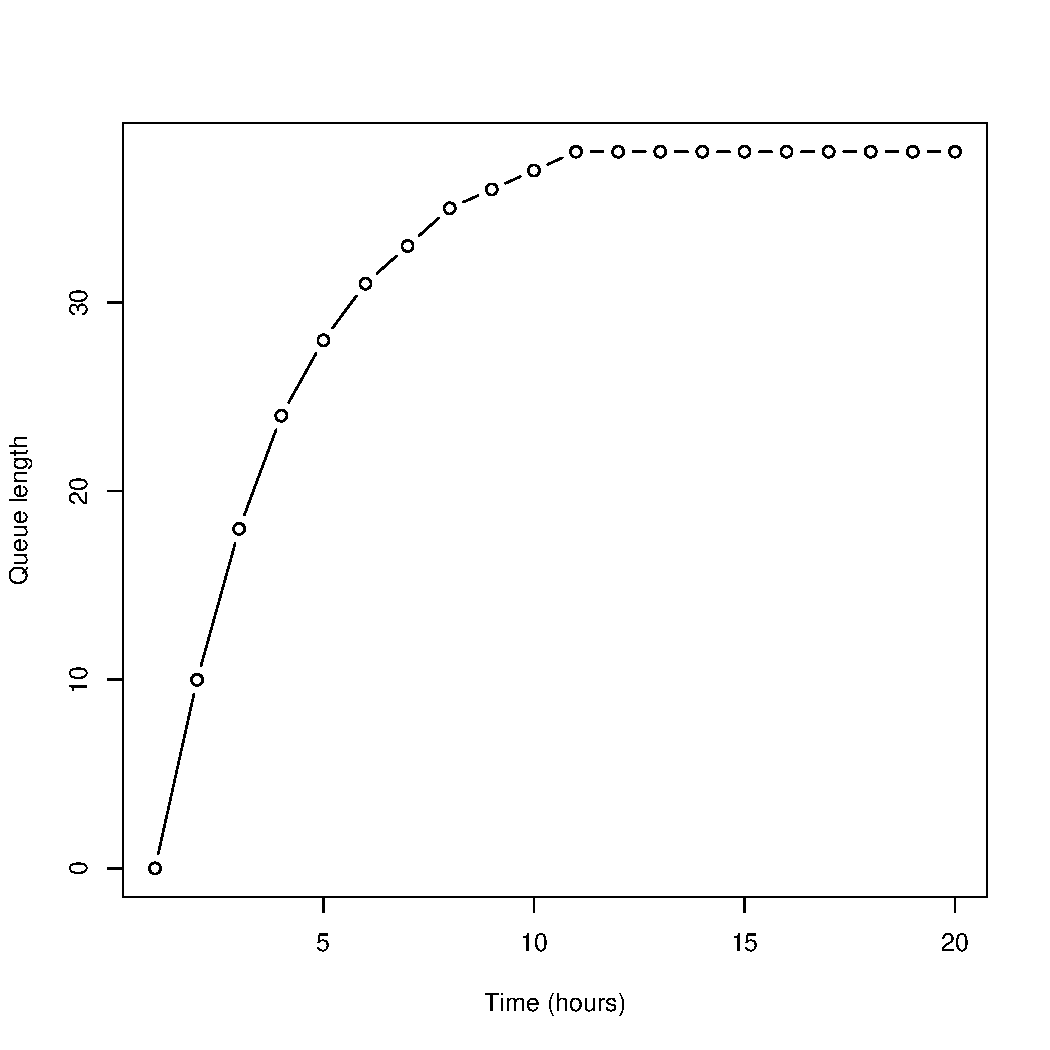
\includegraphics[width=\maxwidth]{figure/firstPlot} 

\end{knitrout}

\begin{figure}
  \begin{center}
\begin{knitrout}
\definecolor{shadecolor}{rgb}{0.969, 0.969, 0.969}\color{fgcolor}
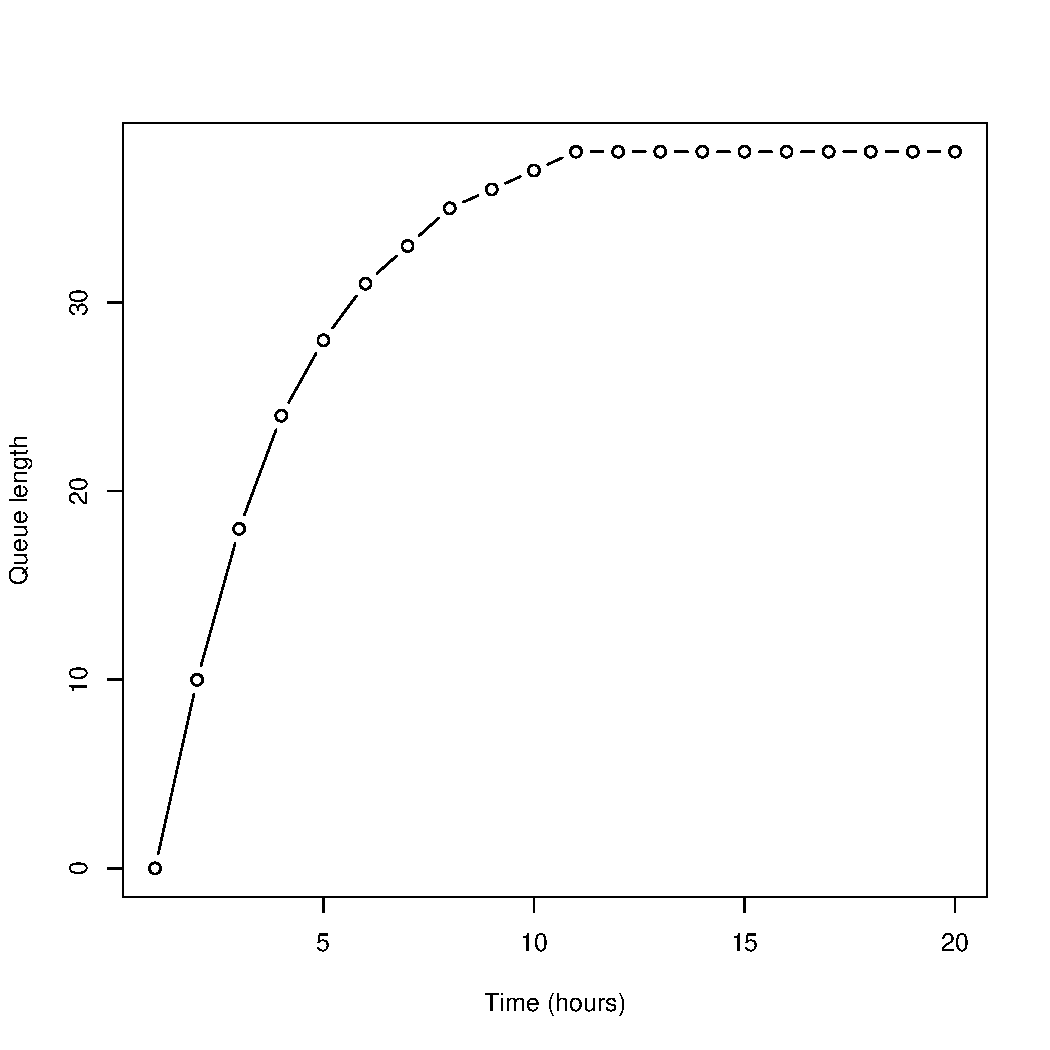
\includegraphics[width=\maxwidth]{figure/qfig1} 

\end{knitrout}
\end{center}
\caption{Queue length ``simulation'': $N(t)=N(t-1)-0.25 \cdot \mbox{round}(N(t-1)+10$.}
\label{fig:queue1}
\end{figure}

\begin{figure}
\begin{center}
\begin{knitrout}
\definecolor{shadecolor}{rgb}{0.969, 0.969, 0.969}\color{fgcolor}
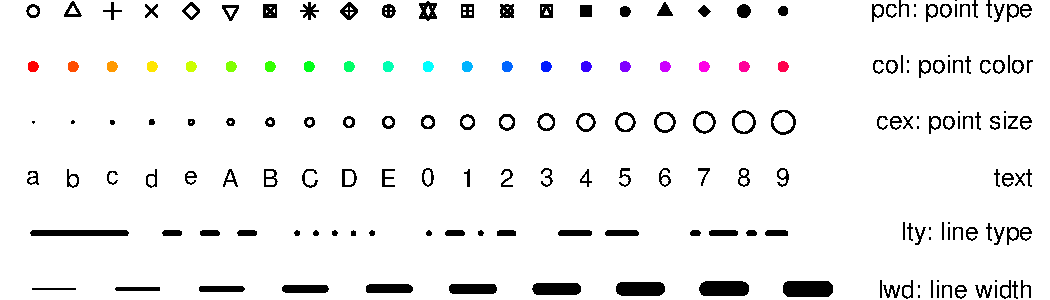
\includegraphics[width=\maxwidth]{figure/chlorfig1} 

\end{knitrout}
\end{center}
\caption{Some of \R's graphics parameters.
Color specification, \code{col}, also applies in many other contexts:
colors are set to a rainbow scale here.  
See \code{?par}
for (many more) details on graphics parameters,
and one or more of \code{?rgb}, \code{?palette},
or \code{apropos("color")} for more on colors.}
\label{fig:graphparms}
\end{figure}

\R's default plotting character is an open circle.
Open symbols are good for plotting large data sets
because it is easier to see where they
overlap, but you could include \code{pch=16} in the
\code{plot} command if you wanted closed circles instead.
Figure~\ref{fig:graphparms} shows several more
ways to adjust the appearance of lines
and points in \R.

\section{\R-markdown}

\R-markdown is a useful tool for reporting your findings.
Essentially, \R-markdown allows you to combine descriptions in English
(or any other natural language) with your \R\ scripts, and \R\ output
in a single document.  Fortunately, RStudio makes \R-markdown very
easy! Currently, \code{html}, \code{pdf}, and \code{docx} formats are
supported by RStudio (\code{html} is least likely to cause problems,
so please use this unless otherwise instructed).  \textbf{You will be
  required to submit all of your assignments using \R-markdown, so
  please take a few moments to get it working on your system now}.

To begin, select \code{File: New: R Markdown...} and follow the
instructions.  Choose an \code{html} document for now.  At this point,
RStudio will probably recommend that you install several add-on
packages -- you should follow this advice.  If everything goes well, a
sample document will open up.  To test that it works, click on the
\includegraphics[scale=0.7]{../icons/knitIcon} icon and an \code{html}
document should appear.  That's it for now.  \textbf{Please email
  either David or Steve if something goes wrong with setting up
  \R-markdown.}

The template \R-markdown file provided by RStudio looks something like
this,
\begin{verbatim}
---
title: "testing"
output: html_document
---

This is an R Markdown document. Markdown is a simple formatting syntax
for authoring HTML, PDF, and MS Word documents. For more details on
using R Markdown see <http://rmarkdown.rstudio.com>.

When you click the **Knit** button a document will be generated that
includes both content as well as the output of any embedded R code
chunks within the document. You can embed an R code chunk like this:

```{r}
summary(cars)
```

You can also embed plots, for example:

```{r, echo=FALSE}
plot(cars)
```

Note that the `echo = FALSE` parameter was added to the code chunk to
prevent printing of the R code that generated the plot.
\end{verbatim}

Notice how this document combines English sentences (e.g. ``This is
an...'') with \R\ code (e.g. \code{summary(cars)}).  When you fit
\code{knit HTML}, the \R\ code is evaluated and displayed with the
documentation provided.  To learn about the \R-markdown format, you
can find help by clicking
the \includegraphics[scale=0.7]{../icons/helpIcon} icon.  You will be
presented with two options, \code{Using R Markdown} and \code{Markdown
  Quick Reference} -- both are useful.  The former takes you to a
website with a tutorial, and the latter to a pane within RStudio
giving tips on syntax.  An example \R-markdown file can be found at
FIXME, which illustrates how to write up a homework assignment.  Note
that this example also illustrates how to use the \LaTeX\ language
within \R-Markdown in order to produce beautiful mathematics.  If you
have never heard of \LaTeX, it is a system for typesetting mathematics
(see FIXME for more details).

\section{Script files and data files}
When you are just trying to figure something out, rather than
reporting on your findings, \R\ scripts can be very useful.  Scripts
are series' of commands stored in text files. Open a new script file
in RStudio using the \code{File: New: R Script} menu option.
%\includegraphics{skullcross-tiny} %% too much trouble!!

Most programs for working with models or analyzing data follow a
simple pattern of program parts:
\begin{enumerate}
\item Initialization statements.
\item (Possibly) input some data from a file or the keyboard.
\item Carry out the calculations that you want.
\item Print the results, graph them, or save them to a file.
\end{enumerate}

For example, a script file might
\begin{enumerate}
\item Load some packages, or run another script file that 
  creates some functions (more on functions later). 
\item Read in data from a text file.
\item Fit several statistical models to the data and
  compare them.
\item Graph the results, and save the graph to disk for including
  in your term project. 
\end{enumerate}
Even for relatively simple tasks, script files are useful for building
up a calculation step-by-step, making sure that each part works before
adding on to it.

Tips for working with data and script files
(sounding slightly scary but just trying to help you avoid common
pitfalls):
\begin{itemize}
\item{To tell \R\ where data and script files are located, you 
    can do any one of the following:
    \begin{itemize}
    \item{use the RStudio magic of pointing and clicking!}
    \item{spell out the {\em path}, or file location, explicitly. (Use
        a single forward slash to separate folders
        (e.g. \verb+"c:/My Documents/R/script.R"+):
        this works on all platforms.)}
    \item{use \code{filename=file.choose()} (this works on all
        platforms, but is only useful on Windows and MacOS).}
    \item{change your working directory to wherever the file(s) are located
        using \code{Change dir} in the \code{File} menu (Windows:
        on Mac it's \code{Misc/Change Working Directory});}
    \item{change your working directory to wherever the file(s) are located
        using the \code{setwd} (\textbf{set} \textbf{w}orking \textbf{d}irectory)
        function, e.g. \verb+setwd("c:/temp")+}
    \end{itemize}
    Changing your working directory is more efficient in the long run, if
    you save all the script and data files for a particular project in the
    same directory and switch to that directory when you start work.  }
\item{it's vital that you save your data and script files as
    \emph{plain text} (or sometimes comma-separated) files.  There are
    three things that can go wrong here: (1) if you use a web browser
    to download files, be careful that it doesn't automatically append
    some weird suffix to the files; (2) if your web browser has a
    ``file association'' (e.g. it thinks that all files ending in
    \code{.dat} are Excel files), make sure to save the file as plain
    text, and without any extra extensions; (3) \textbf{never, (never,
      never) use Microsoft Word to edit your data and script files};
    MS Word will try very hard to get you to save them as Word (rather
    than text) files, which will screw them up!}
\item{If you send script files by e-mail, even if you paste them into
    the message as plain text, lines will occasionally get broken in
    different places --- leading to confusion.  Beware.}
\end{itemize}

As a first example, the file \verb+bucketModel.R+ has the commands
from the leaky bucket model, which can be found at
FIXME. \textbf{Important:} before working with an example file, create
a personal copy in some location on your own computer.  We will refer
to this location as your \emph{temp folder}.  The \code{File} tab in
RStudio will help you keep track of the directory structure of your
projects. At the end of a lab session you \emph{must} move files onto
your personal disk (or email them to yourself).

Now open \textbf{your copy} of \verb+bucketModel.R+. In RStudio,
select the entire text of the file and click on
the \includegraphics[scale=0.7]{../icons/runIcon} icon (pro-tip: hovering
over this icon will reveal a hot key). This has the same effect as
entering the commands by hand into the console: they will be executed
and so a graph is displayed with the results. Highlighting specific
pieces of the file allows you to execute script files one piece at a
time (which is useful for finding and fixing errors). The
\code{source} function allows you to run an entire script file, e.g.
\begin{knitrout}
\definecolor{shadecolor}{rgb}{0.969, 0.969, 0.969}\color{fgcolor}\begin{kframe}
\begin{alltt}
\hlstd{> }\hlkwd{source}\hlstd{(}\hlstr{"c:/temp/bucketModel.R"}\hlstd{)}
\end{alltt}
\end{kframe}
\end{knitrout}

\textbf{Exercise\exnumber} Make a copy of \verb+bucketModel.R+ under a
new name, and modify the copy so that it picks the number of new
arrivals from a Poisson distribution with mean 10
(\code{rpois(1, lambda = 10)}) and plots the data appropriately.  (We
will learn about the Poisson distribution later.)  In the ``setup''
phase of your code, use the command \code{set.seed(101)} to initialize
the random number generator so that you get the same answer as I did.
You should end up with a graph that resembles Figure~\ref{Intro1Fig2}.

\begin{figure}
\begin{center}
\begin{knitrout}
\definecolor{shadecolor}{rgb}{0.969, 0.969, 0.969}\color{fgcolor}
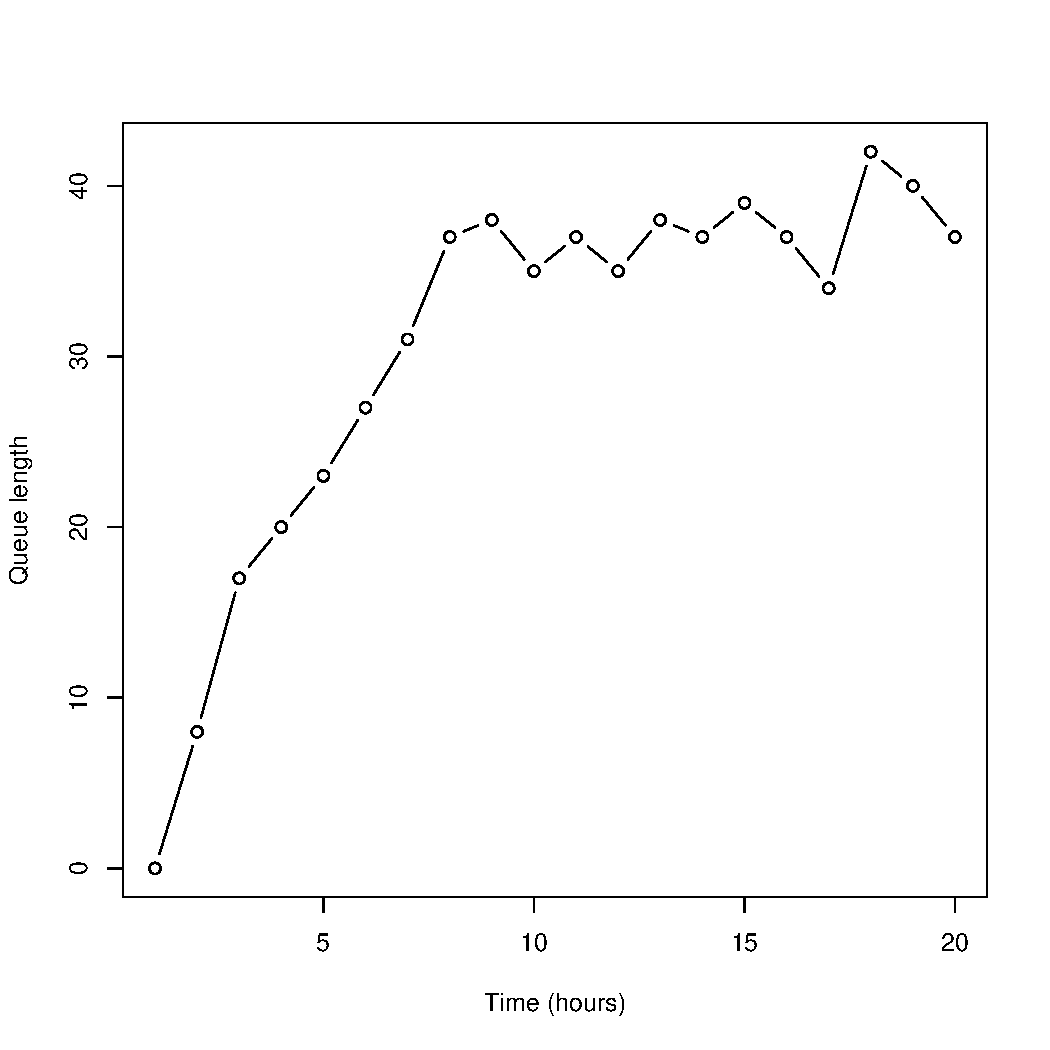
\includegraphics[width=\maxwidth]{figure/unnamed-chunk-2} 

\end{knitrout}
\end{center}
\caption{Queue simulation with random arrivals.}
\label{Intro1Fig2}
\end{figure}

\textbf{Exercise\exnumber} The axes in plots are scaled automatically,
but the outcome is not always ideal (e.g. if you want several graphs
with exactly the same axis limits).  You can use the \code{xlim} and
\code{ylim} arguments in \code{plot} to control the limits:
\begin{knitrout}
\definecolor{shadecolor}{rgb}{0.969, 0.969, 0.969}\color{fgcolor}\begin{kframe}
\begin{alltt}
\hlstd{> }\hlkwd{plot}\hlstd{(x, y,} \hlkwc{xlim} \hlstd{=} \hlkwd{c}\hlstd{(x1, x2), [other stuff])}
\end{alltt}
\end{kframe}
\end{knitrout}
\noindent will draw the graph with the $x$-axis running from \code{x1} to \code{x2}, and using 
\code{ylim = c(y1, y2)} within the \code{plot} command will 
do the same for the $y$-axis. 

Create a plot of queue length versus time with the
$x$-axis running from 0 to 50 and the $y$-axis running from 0 to 50. 

\textbf{Exercise\exnumber} You can place several graphs
within a single figure by using the \code{par} 
function (short for ``parameter'') to adjust the layout of the plot. For example, the 
command
\begin{knitrout}
\definecolor{shadecolor}{rgb}{0.969, 0.969, 0.969}\color{fgcolor}\begin{kframe}
\begin{alltt}
\hlstd{> }\hlkwd{par}\hlstd{(}\hlkwc{mfrow} \hlstd{=} \hlkwd{c}\hlstd{(}\hlnum{2}\hlstd{,} \hlnum{3}\hlstd{))}
\end{alltt}
\end{kframe}
\end{knitrout}
\noindent divides the plotting area into 2 rows and 3 columns. As \R\
draws a series of graphs, it places them along the top row from left
to right, then along the next row, and so on.  \code{mfcol = c(2, 3)}
has the same effect except that \R\ draws successive graphs down the
first column, then down the second column, and so on.

Save \verb+bucketModel.R+ with a new name and modify the program as
follows. Use \code{mfrow = c(1, 2)} to create side-by-side graphs of queue length
vs. time for the deterministic (exactly 10 new people per hour)
and stochastic ($X \sim \mbox{Poisson}(\lambda = 10)$ new people per hour).
Use the \code{ylim} argument to make sure the $y$-axis scales are the
same in each plot.

\textbf{Exercise\exnumber} Use \code{?par} to read about other plot control parameters
that you use \code{par} to set (you should
definitely skim --- this is one of the
longest help files in the whole \R\ system!). 
Then draw a $2 \times 2$ set of plots,
each showing the line $y = 5x + 3$ with $x$ running from 3 to 8, but with 4 different
line styles and 4 different line colors. 

\textbf{Exercise\exnumber} Modify one of your scripts so that
at the very end it saves the plot to disk. Use either
\code{savePlot} or \code{dev.print}.
Use \code{?savePlot}, \code{?dev.print} to read about these functions.  
Note that the argument \code{filename} can include the 
path to a folder; for example, in Windows you can use 
\code{filename="c:/temp/Intro2Figure".}

(These are really exercises in using the help system, with 
the bonus that you learn some things about \code{plot}. (Let's see, 
we know \code{plot} can graph a simulation (\code{N} versus \code{tvec}
and all that). Maybe it can also draw a line to connect the points, or 
just draw the line and leave out the points. That would be useful. So
let's try \code{?plot} and see if it says anything about lines \ldots Hey, it
also says that \code{graphical parameters can be given as arguments to plot},
so maybe I can set line colors inside the plot command instead of using
\code{par} all the time \ldots) 
The help system can be quite helpful (amazingly enough) once
you get used to it and get in the habit of using it often.)

The main point is not to be afraid of experimenting; if you have saved your
previous commands in a script file, there's almost nothing you can break
by trying out commands and inspecting the results.

\textbf{Exercise\exnumber *} Read about \code{lines} and
\code{legend}. Using everything you have learned so far, recreate
Figure 1.5 on pp. 15 of Mooney and Swift's book.  Do not worry if your
graph does not look \emph{exactly} the same, just that it conveys the
same information and uses the same graphical approaches (e.g. line
graph with points; legend).  However, students who come closest to an
exact reproduction will receive a higher mark.

\section{The \R\ package system}
\R\ has many extra packages that provide extra functions.  You are
able to install new packages from a menu within RStudio (\code{Tools:
Install Packages... }). You can also
type
\begin{knitrout}
\definecolor{shadecolor}{rgb}{0.969, 0.969, 0.969}\color{fgcolor}\begin{kframe}
\begin{alltt}
\hlstd{> }\hlkwd{install.packages}\hlstd{(}\hlstr{"plotrix"}\hlstd{)}
\end{alltt}
\end{kframe}
\end{knitrout}
\noindent (for example --- this installs the \code{plotrix} package).
You can install more than one package at a time:
\begin{knitrout}
\definecolor{shadecolor}{rgb}{0.969, 0.969, 0.969}\color{fgcolor}\begin{kframe}
\begin{alltt}
\hlstd{> }\hlkwd{install.packages}\hlstd{(}\hlkwd{c}\hlstd{(}\hlstr{"ellipse"}\hlstd{,} \hlstr{"plotrix"}\hlstd{))}
\end{alltt}
\end{kframe}
\end{knitrout}
\noindent (\code{c} stands for ``combine'', and is the command for
combining multiple things into a single object.)  If the machine on
which you use \R\ is not connected to the Internet, you can download
the packages to some other medium (such as a flash drive) and install
them later, using \code{Install from local zip file} in the menu or
\begin{knitrout}
\definecolor{shadecolor}{rgb}{0.969, 0.969, 0.969}\color{fgcolor}\begin{kframe}
\begin{alltt}
\hlstd{> }\hlkwd{install.packages}\hlstd{(}\hlstr{"plotrix"}\hlstd{,} \hlkwc{repos} \hlstd{=} \hlkwa{NULL}\hlstd{)}
\end{alltt}
\end{kframe}
\end{knitrout}
%\todo{check on other OS}

If you do not have permission to install packages
in \R's central directory, \R\ will
may ask whether you want to install the
packages in a user-specific directory.
Go ahead and say yes.

You will frequently get a warning message 
something like
\code{Warning message: In file.create(f.tg) :
cannot create file '.../packages.html', reason 'Permission denied'}.
Don't worry about this; it means the package has been installed
successfully,
but the main help system index files couldn't be updated
because of file permissions problems.

\section{Statistics in \R}
Some of the important functions and packages (collections
of functions) for statistical modeling and data analysis are summarized in Table 
\ref{StatModelingFunctions}. \cite{MASS} give a 
good practical (although somewhat advanced) overview, and you 
can find a list of available packages and their contents 
at CRAN, the main \R\ website 
(\url{http://www.cran.r-project.org} --- select a mirror site
near you and click on \code{Package sources}). For the most
part, we will not be concerned here with this side of \R.

\begin{table}[t]
\begin{tabular}{p{100pt}p{310pt}}
\hline
\code{aov}, \code{anova} & Analysis of variance or deviance\\
\code{lm} & Linear models (regression, ANOVA, ANCOVA) \\
\code{glm} &  Generalized linear models (e.g. logistic, Poisson regression) \\
\code{gam} & Generalized additive models (in package \code{mgcv}) \\
\code{nls} & Fit nonlinear models by least-squares \\
\code{lme}, \code{nlme},
\code{lmer}, \code{glmer} & Linear,
generalized linear, and nonlinear mixed-effects models (repeated
measures, block effects, spatial models): in packages \code{nlme}
and \code{lme4} \\
\code{boot} & Package: bootstrapping functions \\
\code{splines}  &  Package: nonparametric regression (more in packages
        \code{fields}, \code{KernSmooth}, \code{logspline}, \code{sm} and others)\\
\code{princomp}, \code{manova}, \code{lda}, \code{cancor}
 & Multivariate analysis
(some in package \code{MASS};
also see packages \code{vegan}, \code{ade4}) \\
\code{survival} & Package: survival analysis \\
\code{tree}, \code{rpart} & Packages: tree-based regression \\
\hline 
\end{tabular}
\caption{A few of the functions and packages in \R\ for statistical
modeling and data analysis. There are \emph{many} more, but you will have
to learn about them somewhere else. } 
\label{StatModelingFunctions}
\end{table}

\section{Vectors} 

Vectors and matrices (1- and 2-dimensional rectangular arrays of 
numbers) are pre-defined data types in \R. Operations with vectors 
and matrices may seem a bit abstract now, but we need them to do 
useful things later. 
Vectors' only properties are their type (or \emph{class})
and length, although they can also have an
associated list of names.

We've already seen two ways to create vectors in \R:
\begin{enumerate}
\item{A command in the console window or a script file listing the values, 
such as
\begin{knitrout}
\definecolor{shadecolor}{rgb}{0.969, 0.969, 0.969}\color{fgcolor}\begin{kframe}
\begin{alltt}
\hlstd{> }\hlstd{initialsize} \hlkwb{=} \hlkwd{c}\hlstd{(}\hlnum{1}\hlstd{,} \hlnum{3}\hlstd{,} \hlnum{5}\hlstd{,} \hlnum{7}\hlstd{,} \hlnum{9}\hlstd{,} \hlnum{11}\hlstd{)}
\end{alltt}
\end{kframe}
\end{knitrout}
}
\item{Using \code{read.table}:
\begin{knitrout}
\definecolor{shadecolor}{rgb}{0.969, 0.969, 0.969}\color{fgcolor}\begin{kframe}
\begin{alltt}
\hlstd{> }\hlstd{initialsize} \hlkwb{=} \hlkwd{read.table}\hlstd{(}\hlstr{"c:/temp/initialdata.txt"}\hlstd{)}
\end{alltt}
\end{kframe}
\end{knitrout}
(assuming of course that the file exists in the right place).
}
\end{enumerate}

You can then use a vector in calculations as if it were 
a number (more or less) 
\begin{knitrout}
\definecolor{shadecolor}{rgb}{0.969, 0.969, 0.969}\color{fgcolor}\begin{kframe}
\begin{alltt}
\hlstd{> }\hlstd{(finalsize} \hlkwb{=} \hlstd{initialsize} \hlopt{+} \hlnum{1}\hlstd{)}
\end{alltt}
\begin{verbatim}
## [1]  2  4  6  8 10 12
\end{verbatim}
\begin{alltt}
\hlstd{> }\hlstd{(newsize} \hlkwb{=} \hlkwd{sqrt}\hlstd{(initialsize))}
\end{alltt}
\begin{verbatim}
## [1] 1.000 1.732 2.236 2.646 3.000 3.317
\end{verbatim}
\end{kframe}
\end{knitrout}
(The parentheses are an R trick that tell it to print
out the results of the calculation even though we
assigned them to a variable.)

Notice that \R\ applied each operation to every entry in the vector. 
Similarly, commands like \code{initialsize-5, 2*initialsize, initialsize/10} 
apply subtraction, multiplication, and division to each element of the 
vector. The same is true for 
\begin{knitrout}
\definecolor{shadecolor}{rgb}{0.969, 0.969, 0.969}\color{fgcolor}\begin{kframe}
\begin{alltt}
\hlstd{> }\hlstd{initialsize}\hlopt{^}\hlnum{2}
\end{alltt}
\begin{verbatim}
## [1]   1   9  25  49  81 121
\end{verbatim}
\end{kframe}
\end{knitrout}

In \R\ the default is to apply functions and operations to vectors
in an \emph{element by element} (or ``vectorized'') manner. 

\subsection{Functions for creating vectors}
You can use the \code{seq} function to 
create a set of regularly spaced values.
\code{seq}'s syntax is 
\begin{knitrout}
\definecolor{shadecolor}{rgb}{0.969, 0.969, 0.969}\color{fgcolor}\begin{kframe}
\begin{alltt}
\hlstd{> }\hlstd{x} \hlkwb{<-} \hlkwd{seq}\hlstd{(from, to, by)}
\end{alltt}
\end{kframe}
\end{knitrout}
\noindent or 
\begin{knitrout}
\definecolor{shadecolor}{rgb}{0.969, 0.969, 0.969}\color{fgcolor}\begin{kframe}
\begin{alltt}
\hlstd{> }\hlstd{x} \hlkwb{<-} \hlkwd{seq}\hlstd{(from, to)}
\end{alltt}
\end{kframe}
\end{knitrout}
\noindent or
\begin{knitrout}
\definecolor{shadecolor}{rgb}{0.969, 0.969, 0.969}\color{fgcolor}\begin{kframe}
\begin{alltt}
\hlstd{> }\hlstd{x} \hlkwb{<-} \hlkwd{seq}\hlstd{(from, to, length.out)} \hlcom{# can abbreviate }
\hlstd{> }                               \hlcom{# length.out to length}
\end{alltt}
\end{kframe}
\end{knitrout}
\noindent The first form generates a vector
\code{(from,from+by,from+2*by,...)}  with the last entry not extending
further than than \code{to}.  In the second form the value of
\code{by} is assumed to be 1 or -1, depending on whether \code{from}
or \code{to} is larger.  The third form creates a vector with the
desired endpoints and length.  As we saw above, the syntax
\code{from:to} is a shortcut for \code{seq(from,to)}:
\begin{knitrout}
\definecolor{shadecolor}{rgb}{0.969, 0.969, 0.969}\color{fgcolor}\begin{kframe}
\begin{alltt}
\hlstd{> }\hlnum{1}\hlopt{:}\hlnum{8}
\end{alltt}
\begin{verbatim}
## [1] 1 2 3 4 5 6 7 8
\end{verbatim}
\end{kframe}
\end{knitrout}

\textbf{Exercise\exnumber *} Use \code{seq} to create the vector \code{v=(1 5 9 13)},
and to create a vector going from 1 to 5 in increments of 0.2.

You can use \code{rep} to create a constant vector such as \code{(1 1 1 1)};
the basic syntax is \code{rep(values,lengths)}.  For example,
\begin{knitrout}
\definecolor{shadecolor}{rgb}{0.969, 0.969, 0.969}\color{fgcolor}\begin{kframe}
\begin{alltt}
\hlstd{> }\hlkwd{rep}\hlstd{(}\hlnum{3}\hlstd{,} \hlnum{5}\hlstd{)}
\end{alltt}
\begin{verbatim}
## [1] 3 3 3 3 3
\end{verbatim}
\end{kframe}
\end{knitrout}
\noindent creates a vector in which the value 3 is repeated 5 times. 
\code{rep} will repeat a whole vector multiple times,
\begin{knitrout}
\definecolor{shadecolor}{rgb}{0.969, 0.969, 0.969}\color{fgcolor}\begin{kframe}
\begin{alltt}
\hlstd{> }\hlkwd{rep}\hlstd{(}\hlnum{1}\hlopt{:}\hlnum{3}\hlstd{,} \hlnum{3}\hlstd{)}
\end{alltt}
\begin{verbatim}
## [1] 1 2 3 1 2 3 1 2 3
\end{verbatim}
\end{kframe}
\end{knitrout}
\noindent or will repeat each of the elements in a vector a given
number of times:
\begin{knitrout}
\definecolor{shadecolor}{rgb}{0.969, 0.969, 0.969}\color{fgcolor}\begin{kframe}
\begin{alltt}
\hlstd{> }\hlkwd{rep}\hlstd{(}\hlnum{1}\hlopt{:}\hlnum{3}\hlstd{,} \hlkwc{each} \hlstd{=} \hlnum{3}\hlstd{)}
\end{alltt}
\begin{verbatim}
## [1] 1 1 1 2 2 2 3 3 3
\end{verbatim}
\end{kframe}
\end{knitrout}

Even more flexibly, you can repeat each element in the vector
a different number of times:
\begin{knitrout}
\definecolor{shadecolor}{rgb}{0.969, 0.969, 0.969}\color{fgcolor}\begin{kframe}
\begin{alltt}
\hlstd{> }\hlkwd{rep}\hlstd{(} \hlkwd{c}\hlstd{(}\hlnum{3}\hlstd{,} \hlnum{4}\hlstd{),} \hlkwd{c}\hlstd{(}\hlnum{2}\hlstd{,} \hlnum{5}\hlstd{) )}
\end{alltt}
\begin{verbatim}
## [1] 3 3 4 4 4 4 4
\end{verbatim}
\end{kframe}
\end{knitrout}
The value 3 was repeated 2 times, followed by the value 4 repeated 5 times.
\code{rep} can be a little bit mind-blowing as you get started, but
it will turn out to be useful.

Table \ref{VectorFunctions} lists some of the main functions 
for creating and working with vectors.

\begin{table}[t]
\begin{tabular}
{p{140pt}p{290pt}}
\hline
\code{seq(from, to, by = 1)} & Vector of evenly spaced values, default increment = 1) \\
\code{seq(from, to, length.out)} & Vector of evenly spaced values, specified length) \\
\code{c(u, v, ...) } & Combine a set of numbers and/or vectors into a single vector \\
\code{rep(a, b)} & Create vector by repeating elements of \code{a} by amounts in \code{b} \\
\code{as.vector(x)} & Convert an object of some other type to a vector \\ 
\code{hist(v)} & Histogram plot of value in v \\
\code{mean(v), var(v), sd(v)} & Estimate of mean, variance, standard deviation based on data values in \code{v} \\
\code{cor(v,w)} & Correlation between two vectors \\
\hline
\end{tabular}
\caption{Some important \R\ functions for creating and working with vectors. Many of these have other optional
arguments; use the help system (e.g. \code{?cor}) for more information. The statistical functions such as
\code{var} regard the values as samples from a population and compute an estimate of the population 
statistic; for example \code{sd(1:3)=1}.}
\label{VectorFunctions}
\end{table}

\subsection{Vector indexing}
You will often want to extract a specific 
entry or other part of a vector. This procedure
is called \emph{vector indexing}, and uses
square brackets (\code{[]}):
\begin{knitrout}
\definecolor{shadecolor}{rgb}{0.969, 0.969, 0.969}\color{fgcolor}\begin{kframe}
\begin{alltt}
\hlstd{> }\hlstd{z} \hlkwb{<-} \hlkwd{c}\hlstd{(}\hlnum{1}\hlstd{,} \hlnum{3}\hlstd{,} \hlnum{5}\hlstd{,} \hlnum{7}\hlstd{,} \hlnum{9}\hlstd{,} \hlnum{11}\hlstd{)}
\hlstd{> }\hlstd{z[}\hlnum{3}\hlstd{]}
\end{alltt}
\begin{verbatim}
## [1] 5
\end{verbatim}
\end{kframe}
\end{knitrout}

(how would you use \code{seq} to construct \code{z}?)
\code{z[3]} extracts the third item, or \emph{element}, in the vector \code{z}. 
You can also access a block of elements using the functions for 
vector construction, e.g. 
\begin{knitrout}
\definecolor{shadecolor}{rgb}{0.969, 0.969, 0.969}\color{fgcolor}\begin{kframe}
\begin{alltt}
\hlstd{> }\hlstd{z[}\hlnum{2}\hlopt{:}\hlnum{5}\hlstd{]}
\end{alltt}
\begin{verbatim}
## [1] 3 5 7 9
\end{verbatim}
\end{kframe}
\end{knitrout}
extracts the second through fifth elements.

What happens if you enter \code{v=z[seq(1, 5, 2)]} ? Try it
and see, and make sure you understand what happened. 

You can extracted irregularly spaced elements of a vector. For example
\begin{knitrout}
\definecolor{shadecolor}{rgb}{0.969, 0.969, 0.969}\color{fgcolor}\begin{kframe}
\begin{alltt}
\hlstd{> }\hlstd{z[}\hlkwd{c}\hlstd{(}\hlnum{1}\hlstd{,} \hlnum{2}\hlstd{,} \hlnum{5}\hlstd{)]}
\end{alltt}
\begin{verbatim}
## [1] 1 3 9
\end{verbatim}
\end{kframe}
\end{knitrout}

You can also use indexing to \textbf{set specific values within a vector}. For 
example, 
\begin{knitrout}
\definecolor{shadecolor}{rgb}{0.969, 0.969, 0.969}\color{fgcolor}\begin{kframe}
\begin{alltt}
\hlstd{> }\hlstd{z[}\hlnum{1}\hlstd{]} \hlkwb{=} \hlnum{12}
\end{alltt}
\end{kframe}
\end{knitrout}
changes the value of the first entry in \code{z} while leaving 
all the rest alone, and 
\begin{knitrout}
\definecolor{shadecolor}{rgb}{0.969, 0.969, 0.969}\color{fgcolor}\begin{kframe}
\begin{alltt}
\hlstd{> }\hlstd{z[}\hlkwd{c}\hlstd{(}\hlnum{1}\hlstd{,} \hlnum{3}\hlstd{,} \hlnum{5}\hlstd{)]} \hlkwb{=} \hlkwd{c}\hlstd{(}\hlnum{22}\hlstd{,} \hlnum{33}\hlstd{,} \hlnum{44}\hlstd{)}
\end{alltt}
\end{kframe}
\end{knitrout}
changes the first, third, and fifth values 
(note that we had to use \code{c} to create the vector --- %
can you interpret the error message you get if you
try \code{z[1, 3, 5]} ?)


\textbf{Exercise\exnumber *} Write a \emph{one-line} command to extract 
a vector consisting of the second, first, and third elements of \code{z} 
\emph{in that order}. 

% You may be wondering if vectors in \R\ 
% are row vectors or column vectors (if you don't know what those are,
% don't worry). The answer is ``both and neither''.
% Vectors are printed out as row vectors, but if you use a vector in 
% an operation that succeeds or fails depending on the vector's orientation, 
% \R\ will assume that you want the operation to succeed and will proceed as 
% if the vector has the necessary orientation. For example, \R\ will let
% you add a vector of length 5 to a $5 \times 1$ matrix or to a 
% $1 \times 5$ matrix, in either case yielding a matrix of the 
% same dimensions.

\textbf{Exercise\exnumber} Write a script file that computes values of 
$y=\frac{(x - 1)}{(x + 1)}$ for $x = 1, 2, \cdots, 10$, and plots $y$ versus $x$
with the points plotted and connected by a line (hint:
in \code{?plot}, search for \code{type}).

\textbf{Exercise\exnumber *} The sum of the geometric series $1 + r + r^2 + r^3 + ... + r^n$ 
approaches the limit $1/(1-r)$ for $r < 1$ as $n \rightarrow \infty$.   
Set the values $r=0.5$ and $n=10$, 
and then write a \textbf{one-line} command that creates 
the vector $G = (r^0,r^1,r^2,...,r^n)$. Compare the sum (using \code{sum})
of this vector to the limiting value $1/(1-r)$. 
Repeat for   $n=50$.  (\emph{Note} that comparing very similar numeric values
can be tricky: rounding can happen, and some numbers cannot be represented
exactly in binary (computer) notation.  By default \R\ displays 7~significant
digits (\code{options("digits")}). 
For example:
\begin{knitrout}
\definecolor{shadecolor}{rgb}{0.969, 0.969, 0.969}\color{fgcolor}\begin{kframe}
\begin{alltt}
\hlstd{> }\hlstd{x} \hlkwb{=} \hlnum{1.999999}
\hlstd{> }\hlstd{x}
\end{alltt}
\begin{verbatim}
## [1] 2
\end{verbatim}
\begin{alltt}
\hlstd{> }\hlstd{x} \hlopt{-} \hlnum{2}
\end{alltt}
\begin{verbatim}
## [1] -1e-06
\end{verbatim}
\begin{alltt}
\hlstd{> }\hlstd{x} \hlkwb{=} \hlnum{1.9999999999999}
\hlstd{> }\hlstd{x}
\end{alltt}
\begin{verbatim}
## [1] 2
\end{verbatim}
\begin{alltt}
\hlstd{> }\hlstd{x} \hlopt{-} \hlnum{2}
\end{alltt}
\begin{verbatim}
## [1] -9.992e-14
\end{verbatim}
\end{kframe}
\end{knitrout}
\noindent All the digits are still there, in the second case, but they are not shown.
Also note that \code{x-2} is not exactly $-1 \times 10^{-13}$; this is
unavoidable.)

\subsection{Logical operators}
Logical operators return a 
value of \code{TRUE} or \code{FALSE}. For example, 
try:  
\begin{knitrout}
\definecolor{shadecolor}{rgb}{0.969, 0.969, 0.969}\color{fgcolor}\begin{kframe}
\begin{alltt}
\hlstd{> }\hlstd{a} \hlkwb{=} \hlnum{1}
\hlstd{> }\hlstd{b} \hlkwb{=} \hlnum{3}
\hlstd{> }\hlstd{c} \hlkwb{=} \hlstd{a} \hlopt{<} \hlstd{b}
\hlstd{> }\hlstd{d} \hlkwb{=} \hlstd{(a} \hlopt{>} \hlstd{b)}
\hlstd{> }\hlstd{c}
\end{alltt}
\begin{verbatim}
## [1] TRUE
\end{verbatim}
\begin{alltt}
\hlstd{> }\hlstd{d}
\end{alltt}
\begin{verbatim}
## [1] FALSE
\end{verbatim}
\end{kframe}
\end{knitrout}
\noindent The parentheses around (\verb+a>b+) are optional but make
the code easier to read.
One special case where you \emph{do} need parentheses
(or spaces) is when you make comparisons with negative values;
\verb+a<-1+ will surprise you by setting \code{a=1},
because \code{<-} (representing a left-pointing arrow) is
equivalent to \code{=} in \R.  Use 
\verb+a< -1+, or more safely \verb+a<(-1)+,
to make this comparison.

\begin{table}
\begin{tabular}{p{120pt}p{200pt}}
\hline
\code{x < y}  & less than    \\
\code{x > y}  & greater than \\
\code{x <= y} & less than or equal to \\
\code{x >= y} & greater than or equal to \\
\code{x == y} & equal to \\
\code{x != y} & \emph{not} equal to \\
\hline 
\end{tabular}
\caption{Some comparison operators in \R. Use \code{?Comparison} to learn more.}
\label{Comparisons}
\end{table}

When we compare two vectors or matrices of the same size, or compare a 
number with a vector or matrix, comparisons are done element-by-element.  
For example,
\begin{knitrout}
\definecolor{shadecolor}{rgb}{0.969, 0.969, 0.969}\color{fgcolor}\begin{kframe}
\begin{alltt}
\hlstd{> }\hlstd{x} \hlkwb{=} \hlnum{1}\hlopt{:}\hlnum{5}
\hlstd{> }\hlstd{(b} \hlkwb{=} \hlstd{(x} \hlopt{<=} \hlnum{3}\hlstd{))}
\end{alltt}
\begin{verbatim}
## [1]  TRUE  TRUE  TRUE FALSE FALSE
\end{verbatim}
\end{kframe}
\end{knitrout}
\noindent So if \code{x} and \code{y} are vectors, then \code{(x == y)} will return a vector of 
values giving the element-by-element comparisons. If you want to know
whether \code{x} and \code{y} are identical vectors, use \code{identical(x,y)}
which returns a single value: \code{TRUE} if each entry in \code{x} equals the
corresponding entry in \code{y}, otherwise \code{FALSE}. You can use \code{?Logical} to
read more about logical operators. 
\textbf{Note the difference between = and ==: can you
figure out what happened in the following cautionary tale?}
\begin{knitrout}
\definecolor{shadecolor}{rgb}{0.969, 0.969, 0.969}\color{fgcolor}\begin{kframe}
\begin{alltt}
\hlstd{> }\hlstd{a} \hlkwb{=} \hlnum{1}\hlopt{:}\hlnum{3}
\hlstd{> }\hlstd{b} \hlkwb{=} \hlnum{2}\hlopt{:}\hlnum{4}
\hlstd{> }\hlstd{a} \hlopt{==} \hlstd{b}
\end{alltt}
\begin{verbatim}
## [1] FALSE FALSE FALSE
\end{verbatim}
\begin{alltt}
\hlstd{> }\hlstd{a} \hlkwb{=} \hlstd{b}
\hlstd{> }\hlstd{a} \hlopt{==} \hlstd{b}
\end{alltt}
\begin{verbatim}
## [1] TRUE TRUE TRUE
\end{verbatim}
\end{kframe}
\end{knitrout}
\noindent Exclamation points \verb+!+ are used in \R\ to mean ``not''; 
\verb+!=+ (not \verb+!==+) means ``not equal to''.

\R\ also does arithmetic on logical values, treating \code{TRUE} as 1 and 
\code{FALSE} as 0. So \verb! sum(b) ! returns the value 3, telling us that three 
entries of \code{x} satisfied the condition (\verb+x <= 3+). This is useful for
(e.g.) seeing how many of the elements of a vector are larger than a cutoff
value.

Build more complicated conditions by using \emph{logical operators} to 
combine comparisons: 

\begin{tabular}{cl}
\code{!} &   Negation  \\
\verb!&!, \verb!&&! &     AND  \\
\verb!|!, \verb!||! &     OR 
\end{tabular}

\noindent OR is \emph{non-exclusive}, meaning that \code{x|y} is true 
if either \code{x} or \code{y} \emph{or both} are true
(a ham-and-cheese sandwich would satisfy the condition
``ham OR cheese'').
For example, try
\begin{knitrout}
\definecolor{shadecolor}{rgb}{0.969, 0.969, 0.969}\color{fgcolor}\begin{kframe}
\begin{alltt}
\hlstd{> }\hlstd{a} \hlkwb{=} \hlkwd{c}\hlstd{(}\hlnum{1}\hlstd{,} \hlnum{2}\hlstd{,} \hlnum{3}\hlstd{,} \hlnum{4}\hlstd{)}
\hlstd{> }\hlstd{b} \hlkwb{=} \hlkwd{c}\hlstd{(}\hlnum{1}\hlstd{,} \hlnum{1}\hlstd{,} \hlnum{5}\hlstd{,} \hlnum{5}\hlstd{)}
\hlstd{> }\hlstd{(a} \hlopt{<} \hlstd{b)} \hlopt{&} \hlstd{(a} \hlopt{>} \hlnum{3}\hlstd{)}
\end{alltt}
\begin{verbatim}
## [1] FALSE FALSE FALSE  TRUE
\end{verbatim}
\begin{alltt}
\hlstd{> }\hlstd{(a} \hlopt{<} \hlstd{b)} \hlopt{|} \hlstd{(a} \hlopt{>} \hlnum{3}\hlstd{)}
\end{alltt}
\begin{verbatim}
## [1] FALSE FALSE  TRUE  TRUE
\end{verbatim}
\end{kframe}
\end{knitrout}
\noindent and make sure you understand what happened
(if it's confusing, try breaking up the expression
and looking at the results of \verb+a < b+ and \verb+a > 3+
separately first). The two forms of AND
and OR differ in how they handle vectors. The shorter one does
element-by-element comparisons; the longer one only looks at the
first element in each vector. 

\subsection{Vector indexing II} 
We can also use \emph{logical} vectors (lists of \code{TRUE} and
\code{FALSE} values) to pick elements out of vectors.  This is
important, e.g., for subsetting data (getting rid of those pesky
outliers!)

As a simple example, we might want to focus on just the values $N$
near the maximum in the leaky bucket example:
\begin{knitrout}
\definecolor{shadecolor}{rgb}{0.969, 0.969, 0.969}\color{fgcolor}\begin{kframe}
\begin{alltt}
\hlstd{> }\hlstd{(largeN} \hlkwb{<-} \hlstd{N[N} \hlopt{>} \hlnum{0.9} \hlopt{*} \hlkwd{max}\hlstd{(N)])}
\end{alltt}
\begin{verbatim}
## [1] 38 38 39 42 40
\end{verbatim}
\begin{alltt}
\hlstd{> }\hlstd{(largeN_tvec} \hlkwb{=} \hlstd{tvec[N} \hlopt{>} \hlnum{0.9} \hlopt{*} \hlkwd{max}\hlstd{(N)])}
\end{alltt}
\begin{verbatim}
## [1]  9 13 15 18 19
\end{verbatim}
\end{kframe}
\end{knitrout}
\noindent What is really happening here (think about it for a minute)
is that \verb+N>0.9*max(N)+ generates a logical vector the same length
as \code{N} (\code{FALSE FALSE FALSE \ldots}) which is then used to
select the appropriate values.

If you want the positions at which \code{N} is greater than 90\% of
its maximum, you could say \verb+(1:length(N))[N > 0.9 * max(N)]+, but you
can also use a built-in function: \verb+which(N > 0.9 * max(N))+.  If you
wanted the position at which the maximum value of \code{N} occurs, you
could say \verb+which(N == max(N))+.  (This normally results in a vector
of length 1; when could it give a longer vector?)  There is even a
built-in command for this specific function, \code{which.max}
(although \code{which.max} always returns just the \emph{first}
position at which the maximum occurs).


\textbf{Exercise\exnumber}:
What would happen if instead of setting
\code{largeN} you replaced \code{N}
by saying \verb+N <- N[N > 0.9 * max(N)]+,
and then \verb+tvec <- tvec[N > 0.9 * max(N)]+?
Why would that be wrong?
Try it with some temporary variables --- set
\verb+N2 <- N+ and \verb+tvec2 <- tvec+ 
and then play with \code{N2} and \code{tvec2}
so you don't mess up your working variables ---
and work out what happened \ldots

We can also combine logical operators (making sure to
use the element-by-element \verb+&+ and \verb+|+ versions
of AND and OR):
\begin{knitrout}
\definecolor{shadecolor}{rgb}{0.969, 0.969, 0.969}\color{fgcolor}\begin{kframe}
\begin{alltt}
\hlstd{> }\hlstd{N[N} \hlopt{>} \hlnum{0.9} \hlopt{*} \hlkwd{max}\hlstd{(N)} \hlopt{&} \hlstd{tvec} \hlopt{>=} \hlnum{15}\hlstd{]}
\end{alltt}
\begin{verbatim}
## [1] 39 42 40
\end{verbatim}
\begin{alltt}
\hlstd{> }\hlstd{tvec[N} \hlopt{>} \hlnum{0.9} \hlopt{*} \hlkwd{max}\hlstd{(N)} \hlopt{&} \hlstd{tvec} \hlopt{>=} \hlnum{15}\hlstd{]}
\end{alltt}
\begin{verbatim}
## [1] 15 18 19
\end{verbatim}
\end{kframe}
\end{knitrout}
\noindent If we were going to do this a lot, we could save typing by
assigning a logical vector
\begin{knitrout}
\definecolor{shadecolor}{rgb}{0.969, 0.969, 0.969}\color{fgcolor}\begin{kframe}
\begin{alltt}
\hlstd{> }\hlstd{bigN} \hlkwb{<-} \hlstd{N} \hlopt{>} \hlnum{0.9} \hlopt{*} \hlkwd{max}\hlstd{(N)} \hlopt{&} \hlstd{tvec} \hlopt{>=} \hlnum{15}
\end{alltt}
\end{kframe}
\end{knitrout}
\noindent and using it to do the indexing.

\textbf{Exercise\exnumber} 
\code{runif(n)} is a function (more on it soon) that
generates a vector of \code{n} random, uniformly distributed
numbers between 0 and 1.  
Create a vector of 20 numbers,
then select the subset of those numbers that 
is less than the mean. (If you want your answers to
match mine exactly, use \code{set.seed(273)} to
set the random-number generator to a particular
starting point before you use \code{runif};
[273 is an arbitrary number I chose].)

\textbf{Exercise\exnumber *} 
Find the \emph{positions} 
of the elements that are less than the mean
of the vector you just created (e.g. if your vector were
\verb+(0.1 0.9. 0.7 0.3)+ the answer
would be \verb+(1 4)+).

As I mentioned in passing above, vectors can have
names associated with their elements: if they do,
you can also extract elements by name (use
\code{names} to find out the names).

\begin{knitrout}
\definecolor{shadecolor}{rgb}{0.969, 0.969, 0.969}\color{fgcolor}\begin{kframe}
\begin{alltt}
\hlstd{> }\hlstd{x} \hlkwb{=} \hlkwd{c}\hlstd{(}\hlkwc{first} \hlstd{=} \hlnum{7}\hlstd{,} \hlkwc{second} \hlstd{=} \hlnum{5}\hlstd{,} \hlkwc{third} \hlstd{=} \hlnum{2}\hlstd{)}
\hlstd{> }\hlkwd{names}\hlstd{(x)}
\end{alltt}
\begin{verbatim}
## [1] "first"  "second" "third"
\end{verbatim}
\begin{alltt}
\hlstd{> }\hlstd{x[}\hlstr{"first"}\hlstd{]}
\end{alltt}
\begin{verbatim}
## first 
##     7
\end{verbatim}
\begin{alltt}
\hlstd{> }\hlstd{x[}\hlkwd{c}\hlstd{(}\hlstr{"third"}\hlstd{,} \hlstr{"first"}\hlstd{)]}
\end{alltt}
\begin{verbatim}
## third first 
##     2     7
\end{verbatim}
\end{kframe}
\end{knitrout}

Finally, it is sometimes handy to be able to drop a
particular set of elements, rather than taking a
particular set: you can do this with negative indices.
For example, \code{x[-1]} extracts all but the first
element of a vector.

\textbf{Exercise\exnumber *}:
Specify two ways to take only the elements
in the odd positions (first, third, \ldots)
of a vector of arbitrary length.

\section{Matrices}
\subsection{Creating matrices}
Like vectors, you can create matrices by 
using \code{read.table} to read in 
values from a data file.  (Actually, this
creates a data frame, which is \emph{almost}
the same as a matrix --- see section~\ref{sec:dataframes}.)
You can also create matrices of numbers by creating a vector of the matrix 
entries, and then reshaping them to the desired number of rows
and columns using the function \code{matrix}. For example 
\begin{knitrout}
\definecolor{shadecolor}{rgb}{0.969, 0.969, 0.969}\color{fgcolor}\begin{kframe}
\begin{alltt}
\hlstd{> }\hlstd{(X} \hlkwb{=} \hlkwd{matrix}\hlstd{(}\hlnum{1}\hlopt{:}\hlnum{6}\hlstd{,} \hlkwc{nrow} \hlstd{=} \hlnum{2}\hlstd{,} \hlkwc{ncol} \hlstd{=} \hlnum{3}\hlstd{))}
\end{alltt}
\begin{verbatim}
##      [,1] [,2] [,3]
## [1,]    1    3    5
## [2,]    2    4    6
\end{verbatim}
\end{kframe}
\end{knitrout}
\noindent takes the values 1 to 6 and reshapes them into a 2 by 3 matrix.

By default \R\ loads the values into
the matrix \emph{column-wise} (this is
probably counter-intuitive since we're used
to reading tables row-wise). 
Use the optional
parameter \code{byrow} to change this behavior. 
For example :
\begin{knitrout}
\definecolor{shadecolor}{rgb}{0.969, 0.969, 0.969}\color{fgcolor}\begin{kframe}
\begin{alltt}
\hlstd{> }\hlstd{(A}\hlkwb{=}\hlkwd{matrix}\hlstd{(}\hlnum{1}\hlopt{:}\hlnum{9}\hlstd{,} \hlkwc{nrow} \hlstd{=} \hlnum{3}\hlstd{,} \hlkwc{ncol} \hlstd{=} \hlnum{3}\hlstd{,} \hlkwc{byrow} \hlstd{=} \hlnum{TRUE}\hlstd{))}
\end{alltt}
\begin{verbatim}
##      [,1] [,2] [,3]
## [1,]    1    2    3
## [2,]    4    5    6
## [3,]    7    8    9
\end{verbatim}
\end{kframe}
\end{knitrout}

\R\ will re-cycle through entries in the data vector, if necessary
to fill a matrix of the specified size. So for example
\begin{knitrout}
\definecolor{shadecolor}{rgb}{0.969, 0.969, 0.969}\color{fgcolor}\begin{kframe}
\begin{alltt}
\hlstd{> }\hlkwd{matrix}\hlstd{(}\hlnum{1}\hlstd{,} \hlkwc{nrow} \hlstd{=} \hlnum{10}\hlstd{,} \hlkwc{ncol} \hlstd{=} \hlnum{10}\hlstd{)}
\end{alltt}
\end{kframe}
\end{knitrout}
\noindent creates a 10$\times$10 matrix of ones.

\textbf{Exercise\exnumber} Use a command of the form \code{X =
  matrix(v, nrow = 2, ncol = 4)}
where \code{v} is a data vector, to create the following matrix \code{X}:
\begin{knitrout}
\definecolor{shadecolor}{rgb}{0.969, 0.969, 0.969}\color{fgcolor}\begin{kframe}
\begin{verbatim}
##      [,1] [,2] [,3] [,4]
## [1,]    1    1    1    1
## [2,]    2    2    2    2
\end{verbatim}
\end{kframe}
\end{knitrout}
\noindent If you can, try to use R commands to construct the vector
rather than typing out all of the individual values.

\R\ will also collapse a matrix to behave like a vector
whenever it makes sense: for example \code{sum(X)} above
is 12.

\textbf{Exercise\exnumber} Use \code{rnorm} 
(which is like \code{runif}, but generates Gaussian
(normally distributed) numbers with a specified
mean and standard deviation instead) and \code{matrix} to 
create a $5 \times 7$ matrix of Gaussian random numbers with
mean 1 and standard deviation 2. (Use \code{set.seed(273)}
again for consistency.)

Another useful function for creating matrices is \code{diag}.
\code{diag(v,n)} creates an $n \times n$ matrix with data
vector $v$ on its diagonal. So for example \code{diag(1, 5)}
creates the $5 \times 5$ \emph{identity matrix}, which has 1's on
the diagonal and 0 everywhere else.
Try \code{diag(1:5, 5)} and \code{diag(1:2, 5)}; why does
the latter produce a warning?

Finally, you can use the \code{data.entry} function.  This function
can only edit existing matrices, but for example (try this now!!)
\begin{knitrout}
\definecolor{shadecolor}{rgb}{0.969, 0.969, 0.969}\color{fgcolor}\begin{kframe}
\begin{alltt}
\hlstd{> }\hlstd{A}\hlkwb{=}\hlkwd{matrix}\hlstd{(}\hlnum{0}\hlstd{,} \hlkwc{nrow} \hlstd{=} \hlnum{3}\hlstd{,} \hlkwc{ncol} \hlstd{=} \hlnum{4}\hlstd{)}
\hlstd{> }\hlkwd{data.entry}\hlstd{(A)}
\end{alltt}
\end{kframe}
\end{knitrout}
\noindent will create \code{A} as a $3 \times 4$ matrix, and then call
up a spreadsheet-like interface in which you can change the values to
whatever you need.

\begin{table}[t]
\begin{tabular}{p{145pt}p{290pt}}
\hline
\code{matrix(v, nrow = m, ncol = n)} & $m \times n$ matrix using the values in \code{v} \\
\code{t(A)} & transpose (exchange rows and columns) of matrix \code{A} \\
\code{dim(X)} & dimensions of matrix X. \code{dim(X)[1]}=\# rows, \code{dim(X)[2]}=\# columns \\
\code{data.entry(A)} & call up a spreadsheet-like interface to edit the values in \code{A} \\
\code{diag(v, n)} & diagonal $n \times n$ matrix with $v$ on diagonal, 0 elsewhere 
(\code{v} is 1 by default, so \code{diag(n)} gives an $n \times n$ identity matrix)\\
\code{cbind(a, b, c, ...)} & combine compatible objects by attaching them along columns \\
\code{rbind(a, b, c, ...)} & combine compatible objects by attaching them along rows \\
\code{as.matrix(x)} & convert an object of some other type to a matrix, if possible \\
\code{outer(v, w)} & ``outer product'' of vectors \code{v}, \code{w}: the matrix whose 
$(i,j)$\textsuperscript{th}
element is \code{v[i]*w[j]} \\
\hline
\end{tabular}
\caption{Some important functions for creating and working with matrices. Many
of these have additional optional arguments; use the help system for full details.}
\label{MatrixFunctions}
\end{table}

\subsection{\code{cbind} and \code{rbind}} 
If their sizes match, you can combine vectors to form matrices, and
stick matrices together with vectors or other matrices.
\code{cbind} (``column bind'') and \code{rbind}
(``row bind'') are the functions to use.

\code{cbind} binds together columns of two objects. One thing it can do
is put vectors together to form a matrix: 
\begin{knitrout}
\definecolor{shadecolor}{rgb}{0.969, 0.969, 0.969}\color{fgcolor}\begin{kframe}
\begin{alltt}
\hlstd{> }\hlstd{(C}\hlkwb{=}\hlkwd{cbind}\hlstd{(}\hlnum{1}\hlopt{:}\hlnum{3}\hlstd{,} \hlnum{4}\hlopt{:}\hlnum{6}\hlstd{,} \hlnum{5}\hlopt{:}\hlnum{7}\hlstd{))}
\end{alltt}
\begin{verbatim}
##      [,1] [,2] [,3]
## [1,]    1    4    5
## [2,]    2    5    6
## [3,]    3    6    7
\end{verbatim}
\end{kframe}
\end{knitrout}
\noindent \R\ interprets vectors as row or column vectors according to
what you're doing with them. Here it treats them as column vectors so that 
columns exist to be bound together. On the other hand, 
\begin{knitrout}
\definecolor{shadecolor}{rgb}{0.969, 0.969, 0.969}\color{fgcolor}\begin{kframe}
\begin{alltt}
\hlstd{> }\hlstd{(D} \hlkwb{=} \hlkwd{rbind}\hlstd{(}\hlnum{1}\hlopt{:}\hlnum{3}\hlstd{,} \hlnum{4}\hlopt{:}\hlnum{6}\hlstd{))}
\end{alltt}
\begin{verbatim}
##      [,1] [,2] [,3]
## [1,]    1    2    3
## [2,]    4    5    6
\end{verbatim}
\end{kframe}
\end{knitrout}
\noindent treats them as rows. Now we have two matrices that can be combined. 

\textbf{Exercise\exnumber} Verify that \code{rbind(C, D)} works,
\code{cbind(C, C)} works, but \code{cbind(C, D)} doesn't. Why not?


\subsection{Matrix indexing}
Matrix indexing is like vector indexing except that you have to
specify both the row and column, or range of rows and columns. For
example \code{z=A[2, 3]} sets \code{z} equal to 6, which is the
(2\textsuperscript{nd} row, 3\textsuperscript{rd} column) entry of the
matrix \textbf{A} that you recently created, and
\begin{knitrout}
\definecolor{shadecolor}{rgb}{0.969, 0.969, 0.969}\color{fgcolor}\begin{kframe}
\begin{alltt}
\hlstd{> }\hlstd{A[}\hlnum{2}\hlstd{,} \hlnum{2}\hlopt{:}\hlnum{3}\hlstd{]}
\end{alltt}
\begin{verbatim}
## [1] 5 6
\end{verbatim}
\begin{alltt}
\hlstd{> }\hlstd{(B} \hlkwb{=} \hlstd{A[}\hlnum{2}\hlopt{:}\hlnum{3}\hlstd{,} \hlnum{1}\hlopt{:}\hlnum{2}\hlstd{])}
\end{alltt}
\begin{verbatim}
##      [,1] [,2]
## [1,]    4    5
## [2,]    7    8
\end{verbatim}
\end{kframe}
\end{knitrout}

There is an easy shortcut to extract entire rows or columns: leave out the limits,
leaving a blank before or after the comma.
\begin{knitrout}
\definecolor{shadecolor}{rgb}{0.969, 0.969, 0.969}\color{fgcolor}\begin{kframe}
\begin{alltt}
\hlstd{> }\hlstd{(first.row}\hlkwb{=}\hlstd{A[}\hlnum{1}\hlstd{,])}
\end{alltt}
\begin{verbatim}
## [1] 1 2 3
\end{verbatim}
\begin{alltt}
\hlstd{> }\hlstd{(second.column}\hlkwb{=}\hlstd{A[,}\hlnum{2}\hlstd{])}
\end{alltt}
\begin{verbatim}
## [1] 2 5 8
\end{verbatim}
\end{kframe}
\end{knitrout}

(What does \code{A[,]} do?)

As with vectors, indexing also works in reverse for assigning values to matrix 
entries. For example,
\begin{knitrout}
\definecolor{shadecolor}{rgb}{0.969, 0.969, 0.969}\color{fgcolor}\begin{kframe}
\begin{alltt}
\hlstd{> }\hlstd{(A[}\hlnum{1}\hlstd{,} \hlnum{1}\hlstd{]} \hlkwb{=} \hlnum{12}\hlstd{)}
\end{alltt}
\begin{verbatim}
## [1] 12
\end{verbatim}
\end{kframe}
\end{knitrout}

You can do the same with blocks, rows, or columns, for example
\begin{knitrout}
\definecolor{shadecolor}{rgb}{0.969, 0.969, 0.969}\color{fgcolor}\begin{kframe}
\begin{alltt}
\hlstd{> }\hlstd{(A[}\hlnum{1}\hlstd{,]}\hlkwb{=}\hlkwd{c}\hlstd{(}\hlnum{2}\hlstd{,} \hlnum{4}\hlstd{,} \hlnum{5}\hlstd{))}
\end{alltt}
\begin{verbatim}
## [1] 2 4 5
\end{verbatim}
\end{kframe}
\end{knitrout}

If you use \code{which} on a matrix, \R\ will normally
treat the matrix as a vector --- so for example
\code{which(A==8)} will give the answer 6 (figure out
why).  However, \code{which} does have an 
option that will treat its argument
as a matrix:
\begin{knitrout}
\definecolor{shadecolor}{rgb}{0.969, 0.969, 0.969}\color{fgcolor}\begin{kframe}
\begin{alltt}
\hlstd{> }\hlkwd{which}\hlstd{(A}\hlopt{==}\hlnum{8}\hlstd{,}\hlkwc{arr.ind}\hlstd{=}\hlnum{TRUE}\hlstd{)}
\end{alltt}
\begin{verbatim}
##      row col
## [1,]   3   2
\end{verbatim}
\end{kframe}
\end{knitrout}

\section{Other structures: Lists and data frames}

\subsection{Lists}
While vectors and matrices may seem familiar,
lists are probably new to you.
Vectors and matrices have to contain elements that
are all the same type:
lists in \R\ can contain anything --- vectors, matrices,
other lists \ldots
Indexing lists is a little different too: use
double square brackets \code{[[ ]]} (rather
than single square brackets as for a vector)
to extract an element of a list by number or name, or
\verb+$+ to extract an element by name (only).
Given a list like this:
\begin{knitrout}
\definecolor{shadecolor}{rgb}{0.969, 0.969, 0.969}\color{fgcolor}\begin{kframe}
\begin{alltt}
\hlstd{> }\hlstd{L} \hlkwb{=} \hlkwd{list}\hlstd{(}\hlkwc{A} \hlstd{= x,} \hlkwc{B} \hlstd{= y,} \hlkwc{C} \hlstd{=} \hlkwd{c}\hlstd{(}\hlstr{"a"}\hlstd{,} \hlstr{"b"}\hlstd{,} \hlstr{"c"}\hlstd{))}
\end{alltt}
\end{kframe}
\end{knitrout}
\noindent Then \verb+L$A+, \verb+L[["A"]]+, and 
\verb+L[[1]]+ will all grab the first element
of the list.

You won't use lists too much at the beginning,
but many of R's own results are structured in
the form of lists.

\subsection{Data frames}
\label{sec:dataframes}

Data frames are the solution to the problem that most data sets have
several different kinds of variables observed for each sample
(e.g. categorical site location and continuous rainfall), but matrices
can only contain a single type of data.  Data frames are a hybrid of
lists and vectors; internally, they are a list of vectors that may be
of different types but must all be the same length, but you can do
most of the same things with them (e.g., extracting a subset of rows)
that you can do with matrices.  You can index them either the way you
would index a list, using \verb+[[ ]]+ or \verb+$+ --- where each
variable is a different item in the list --- or the way you would
index a matrix.  Use \code{as.matrix} if you have a data frame (where
all variables are the same type) that you really want to be a matrix,
e.g. if you need to transpose it (use \code{as.data.frame} to go the
other way).


\bibliography{lab1.bib}
\bibliographystyle{plain}

\end{document}
